\input{header}
\bibliographystyle{jureco}
\title{Entwicklung eines Vorgehensmodells für Cloud-Migrationen zu Salesforce}

\subtitle{SUBTITEL}

\subsubtitle{Bachelorthesis
\linebreak Claus Steffen Pegenau (1933040)}


\setinstitutionlogo[width]{images/ise_logo.pdf}
%\referee{Gutachter 1}{Gutachter 2}








\newcommand{\titel}{Entwicklung eines Vorgehensmodells für Cloud-Migrationen zu 
Salesforce}
\newcommand{\untertitel}{Eine Betrachtung aus Sicht eines Independent Software 
Vendors}
\newcommand{\abgabedatum}{15.03.2017}

\usepackage{enumitem}
\usepackage{multirow}
\usepackage{soul}
\usepackage{amsthm}
\newtheorem*{cloudcomputing}{Cloud-Computing}

\begin{document}
\noindent
\setstretch{1.2}
\maketitle

\urlstyle{same}
\pagenumbering{roman}
%
%
%Die erste Seite der Arbeit mit Angaben zum Verfasser, zum Lehrstuhl und zum Thema
%
%

\singlespacing 
\noindent Technische Universität Darmstadt \\\\
Fachbereich Rechts- und Wirtschaftswissenschaften \\\\
Fachgebiet Wirtschaftsinformatik -- Information Systems \& Electronic Services \\\\
Prof. Dr. Alexander Benlian \\\\
Betreuer: Prof. Dr. Alexander Benlian \\\\
\\
\lbrack Bachelorthesis\rbrack zu dem Thema: \\\\
\lbrack THEMA\rbrack \\\\
\lbrack SUBTITEL\rbrack \\\\
\\
Bearbeitet von: Claus Steffen Pegenau \\\\
Matr.-Nr.: 1933040 \\\\
Studiengang: Wirtschaftsinformatik \\\\
Eingereicht am: \lbrack XXX\rbrack \\\\

\onehalfspacing

%\newpage
%\thispagestyle{empty}
\setcounter{page}{2}
%
%
%Ehrenwörtliche Erklärung
%
%

\section*{Förmliche Erklärung}
%\thispagestyle{empty}
Hiermit erkläre ich, Claus Steffen Pegenau, geboren am 16.03.1990, an Eides 
statt, dass ich die vorliegende Bachelorthesis ohne 
fremde Hilfe und nur unter Verwendung der zulässigen Mittel sowie der 
angegebenen Literatur angefertigt habe.
\\
\\
Die Arbeit wurde bisher keiner anderen Prüfungsbehörde vorgelegt und auch noch
nicht veröffentlicht.
\\
\vspace*{4.5cm}
\\

\noindent Darmstadt, den \abgabedatum
\\
\vspace*{3.5cm}\\
\underline{~~~~~~~~~~~~~~~~~~~~~~~~~~~~~~~~~~~~~~~~~~~~~~~~~~~~~~~~~~~~~~~~~~~~~~~~}\\(Unterschrift)
\normalsize


%\newpage %Dieser Befehl muss hinzugefügt werden, falls man "twoside" anstatt "oneside" als Dokumentenoption benutzt
%\thispagestyle{empty} %Dieser Befehl muss hinzugefügt werden, falls man "twoside" anstatt "oneside" als Dokumentenoption benutzt


\pagestyle{headings}
        
\tableofcontents	
\newpage 
\listoffigures
\newpage
\listoftables
\clearpage
\setstretch{1.2}

\newcounter{seitenzahlroemisch}
\setcounter{seitenzahlroemisch}{\value{page}}

\pagenumbering{arabic}
\section{Einleitung}
%\lbrack Zitat (optional)\rbrack :
%\begin{quote}
%\glqq Was ist die Absicht eines wissenschaftlichen Buches? Es stellt Gedanken 
%dar und will den Leser von ihrer Gültigkeit überzeugen. Darüber hinaus will 
%der Leser auch wissen: woher kommen diese Gedanken und wohin führen sie? Mit 
%welchen Richtungen auf anderen Gebieten hängen sie zusammen?\grqq
%\pcite{}{XVII}{carnap1974}
%\end{quote}
Die Cloud ist im Mainstream angekommen. \pcite{}{}{thoughtsOnCloud} Wie in 
Abbildung ~\ref{umsatz_cloud_computing_weltweit} darsgestellt, wuchs der 
weltweite Umsatz mit Cloud-Computing von 58,6 Milliarden US-Dollar im 
Jahr 2009 auf geschätzte 203,9 Milliarden US-Dollar im Jahr 2016, was einem 
durchschnittlichen jährlichen Wachstum von 16,87\%\footnote{CAGR(2009,2016) = 
16,87\%} entspricht. \pcite{}{}{CloudUmsatzWeltweit} \\
Auch deutsche Unternehmen drängen zunehmend in die Cloud. Das 
Marktforschungsunternehmen PAC schätzt, dass der 
deutsche Cloud-Markt im Jahr 2016 eine Größe von 12,5 Milliarden Euro hatte und 
mit durchschnittlich jährlich 20,9\%\footnote{CAGR(2016,2020) = 20,9\%} auf 31,4 
Milliarden im Jahr 2020 anwächst. Im deutlichen Gegensatz dazu prognostiziert 
PAC für den Markt der traditionellen IT-Dienstleistungen ein negatives Wachstum 
von  -1,7\%\footnote{CAGR(2015,2019) = -1,7\%}. \pcite{}{}{MarketVision}

\begin{figure}[bh]
\begin{center}
\begin{tikzpicture}
\begin{axis}[
/pgf/number format/.cd,
        use comma,
        1000 sep={},
    %title={Prognose zum Umsatz mit Cloud Computing weltweit von 2009 bis 2016},
    xlabel={Jahr},
    ylabel={Umsatz [Milliarden US-Dollar]},
	axis y line=left,
	axis x line=middle,
every axis x label/.style={at={(current axis.right of origin)},anchor=west},
every axis y label/.style={at={(current axis.north west)},above=2mm},
    xmin=2008, xmax=2017,
    ymin=0, ymax=230,
    %xtick={0,20,40,60,80,100},
    %ytick={0,20,40,60,80,100,120},
    legend pos=north west,
    ymajorgrids=true,
    grid style=dashed
]

\addplot[color=blue,mark=square,]
    coordinates {
	(2009,58.6)
	(2010,76.94)
	(2011,92.97)
	(2012,110.27)
	(2013,130.7)
	(2014,153.91)
	(2015,175)
	(2016,203.9)
    };
    %{Cloud Umsatz weltweit}
    
%\addplot[color=green,mark=square,]
%    coordinates {
%    
%(2009,0)(2010,0)(2011,0)(2012,2.267)(2013,3.050)(2014,4.071)(2015,5.374)(2016
% ,6.667)
%    };
    %\legend{Salesforce}
 
\end{axis}
\end{tikzpicture} 
\caption{Prognose zum Umsatz mit Cloud Computing weltweit von 2009 bis 2015 mit 
geschätztem Wert für 2016 entnommen aus \cite{CloudUmsatzWeltweit} }
\label{umsatz_cloud_computing_weltweit}

\end{center}
\end{figure}


Gerade Softwarehersteller aus diesem traditionellen Bereich der 
IT-Dienstleistungen sehen sich unter Druck gesetzt, ihre 
Unternehmungen von diesem schrumpfenden Markt weg, in den stark wachsenden 
Cloud-Markt zu verlagern. Dabei ist es intuitiv vernünftig, vorhandene 
Kernkompetenzen durch Migrationen bestehender Produkte zu nutzen, um 
Wettbewerbsvorteile auf dem neuen Markt zu erlangen. \\
Doch nicht nur die Umsatzentwicklung des Marktes setzt die Softwarehersteller 
unter Druck: Ihre Kunden haben sich an Anwendungen in der Cloud gewöhnt und
erwarten sich - von ihr - eine günstigere, schnellere, einfachere, flexiblere 
und effizientere IT im Allgemeinen. \pcite{}{}{economics_of_the_cloud}
\begin{comment}
Günstiger, weil bei der Beschaffung, der Wartung und dem 
Betrieb des Rechenzentrums Skalenerträge erzielt werden können. Schneller, weil 
Cloud-Anbieter Leistungsreserven in einem Umfang bilden können und müssen, wie 
es für einzelne Firmen in ihren IT-Landschaften kaum möglich ist. Einfacher, 
weil Cloud-Dienste in der Regel auch mit Mobilgeräten gut bedienbar sind. 
Flexibler, weil sich Leistungen unkompliziert über das Internet buchen lassen 
und automatisch skalieren. Effizienter, weil nur der Umfang bezahlt wird, 
der auch genutzt wird. \pcite{}{}{economics_of_the_cloud} \\ 
\end{comment}

Diese bei den Nutzern geweckten Erwartungen sorgen bei den Softwareherstellern 
für zusätzlichen Migrationsdruck, sie setzen aber auch einen neuen, höheren 
Maßstab für Software im Allgemeinen.

Entschließt sich ein Softwarehersteller dazu, seine Produkte 
als Dienstleistungen in der Cloud anzubieten, ändert sich nicht nur die 
technologische, sondern auch die wirtschaftliche Umgebung erheblich, da ein 
neuer Markt erschlossen wird und bedacht werden muss, wie und wo die 
Cloud-Lösung auf dem Markt zu positionieren ist. Die Position im Wettbewerb hat 
nicht nur für das Vertriebsmodell  Auswirkungen - man 
denke an Fragen der Lizenzierung und Preismodelle - sondern auch den 
Leistungsumfang. Denn je standardisierter eine Software ist, je 
geringer die nötige Anpassbarkeit, desto wahrscheinlicher lassen sich bei einem 
Betrieb in der 
Cloud die genannten Vorteile realisieren. \pcite{}{}{saasBuxmann2008} Dies 
hängt damit zusammen, dass sich bei standardisierter Software Stellschrauben 
vor dem Nutzer verbergen lassen. Im Optimalfall spielen Netzwerktopologie, 
Betriebssystem, Laufzeitumgebung und Datenbanken keine Rolle; der Anwender 
sieht und arbeitet lediglich mit der Software. In diesem Fall spricht man von 
"`Software as a Service"' (SaaS). \pcite{}{11}{economics_of_the_cloud}


\begin{comment}
Als SaaS-Vertriebsplattform soll in dieser Arbeit schwerpunktmäßig Salesforce 
betrachtet werden, das mit "`AppExchange"' einen Marktplatz zur Verfügung 
stellt, auf dem Hersteller ihre auf der Salesforceplattform laufenden 
Anwendungen anbieten können. Die Konzentration auf Salesforce als Zielplattform 
war zum einen durch das Unternehmen gegeben, mit dem in freundlicher 
Kooperation diese Thesis entstanden ist.

\begin{figure}[bh]
\begin{center}
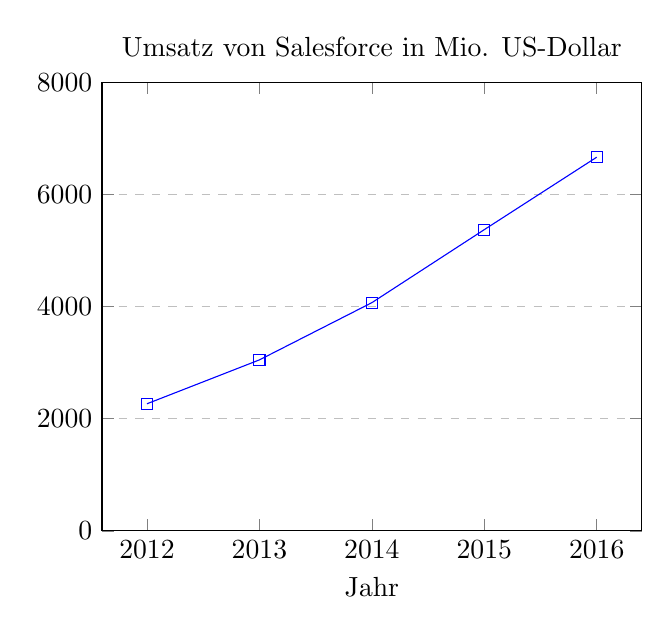
\begin{tikzpicture}
\begin{axis}[
/pgf/number format/.cd,
        use comma,
        1000 sep={},
    title={Umsatz von Salesforce in Mio. US-Dollar},
    xlabel={Jahr},
    %ylabel={Umsatz [Mio. US-Dollar]},
    %xmin=0, xmax=100,
    ymin=0, ymax=8000,
    %xtick={0,20,40,60,80,100},
    %ytick={0,20,40,60,80,100,120},
    legend pos=north west,
    ymajorgrids=true,
    grid style=dashed
]

\addplot[color=blue,mark=square,]
    coordinates {
    (2012,2267)(2013,3050)(2014,4071)(2015,5374)(2016,6667)
    };
    %\legend{Salesforce}
 
\end{axis}
\end{tikzpicture}
\caption{Umsatzzahlen entnommen aus \cite[43]{salesforceannualreport} }
\label{UmsatzzahlenSalesforce}
\end{center}
\end{figure}
Zum anderen aber gehört Salesforce neben Microsoft 
und Google zu den größten SaaS-Anbietern
\pcite{}{247}{softwareindustrie2015} und konnte zwischen 2012 und 2016 
den Umsatz mit durchschnittlich 31\% von 2,267 Milliarden US-Dollar auf 
6,667 Milliarden US-Dollar rasant steigern (Vgl. Abbildung 
~\ref{UmsatzzahlenSalesforce}). Daher dürfte es als Zielplattform für 
viele Unternehmen eine Option sein.
\end{comment}

In der Literatur finden sich zahlreiche Vorgehensmodelle, die 
versuchen, die Migration eines Altsystems beziehungsweise einer Altsoftware 
in die Cloud im 
weitesten Sinne zu strukturieren. In einigen, wie in dem von 
\citeflow{framework_for_architecture-driven_migration} entwickelten Modell wird 
ein technischer Schwerpunkt gesetzt; wirtschaftliche Aspekte bleiben weitgehend 
unberücksichtigt. Andere fokussieren sich lediglich auf den Kosten-Faktor 
(\citeflow{fivephases}). Umfassendere Modelle 
(\citeflow{migrating_applications_to_public_cloud_services}) betonen die 
markt-strategischen Folgen einer Cloud-Migration für Unternehmen. 

Zielgruppe der Modelle sind in der Regel Unternehmen, die Teile ihrer 
IT-Landschaft in die Cloud migrieren wollen. Dies kann zum Beispiel ein 
Unternehmen sein, das 
seine Lagerhaltung in die Cloud verlagern will. Eine in 
dieser Arbeit durchgeführte Literaturrecherche ergab, 
dass Softwarehersteller als Zielgruppe bisher vernachlässigt wurden. Der 
Unterschied zwischen den beiden Gruppen ist gravierend: Während im oben 
genannten Beispiel die 
Lagerhaltung in Form einer Software lediglich das Kerngeschäft unterstützt, 
besteht für den Softwarehersteller das Kerngeschäft in der zu migrierenden 
Software. Für den Erfolg im Wettbewerb ist eine strategische 
Neuausrichtung 
unabdingbar, unterscheidet sich in ihrer Tragweite und ihrem Umfang jedoch 
erheblich von den strategischen Überlegungen, die ein Unternehmen einer anderen 
Branche bei der Cloud Migration treffen muss. 

Um diese Forschungslücke zu schließen, soll ein Modell entwickelt werden, das 
Softwarehersteller bei der Migration in die Cloud unterstützen soll. Grundlage 
ist eine Literaturrecherche, die die folgenden Fragen klären soll:
\begin{enumerate}
	\item Welche Merkmale (Chancen und Risiken) der Cloud sind bei der 
Migration zu berücksichtigen?
	\item Wie beeinflussen die gefundenen Merkmale die strategische 
Ausrichtung und das Geschäftsmodell eines Softwareherstellers?
	\item Wie beeinflussen die gefundenen Merkmale den Migrationsprozess 
eines Softwareherstellers?
\end{enumerate}

Bevor diese Fragen in Kapitel~\ref{cha:entwicklung_vorgehensmodell}  
beantwortet werden und in der Entwicklung eines Vorgehensmodells resultieren, 
wird in Kapitel ~\ref{cha:grundlagen} auf grundlegende Fragen eingegangen: 
Welche Vorteile verspricht die Cloud und wie lassen sie sich erzielen? Auf 
welche Weise unterschiedet sich eine Cloud-Migration von herkömmlichen 
Migrationen in der IT? Was wird in dieser Arbeit unter einem Softwarehersteller 
verstanden und welche Annahmen werden getroffen? Wie wirken sich dessen 
Charakteristika auf die Migration aus?
Um Erfahrungen aus der Praxis in das 
Modell einzubeziehen, wurde das entwickelte Modell in Zusammenarbeit mit einem 
Beratungsunternehmen auf ein reales Projekt angewendet; Unternehmen und Projekt 
werden ebenfalls in diesem Kapitel vorgestellt.
Das Grundlagenkapitel schließt mit der Vorstellung des Fünf-Phasen-Modells, das 
als Basis und Orientierung für das in dieser Arbeit entwickelte Modell dient.

Kapitel~\ref{cha:method} beschreibt die Literaturrecherche mit der die 
Forschungsfragen beantwortet wurden. Um praktische Erfahrungen einfließen zu 
lassen wurden Gespräche mit Mitarbeitern geführt, deren Ablauf ebenfalls in 
diesem Kapitel geschildert werden.

In Kapitel~\ref{cha:result} wird das Vorgehensmodell beispielhaft auf das zu 
migrierende Projekt aus der Praxis angewendet; es werden Möglichkeiten 
dargestellt, um Chancen der Cloud zu realisieren und Risiken zu meiden -- auch 
in Bezug auf das Geschäftsmodell.

In Kapitel~\ref{cha:diskussion} werden die Unterschiede zwischen 
vorgeschlagenem und tatsächlichem Vorgehen herausgearbeitet und diskutiert.

Die Ergebnisse dieser Diskussion werden anschließend in Kapitel~\ref{cha:fazit} 
zusammengefasst, offene Fragestellungen, Herausforderungen und Forschungsfragen 
formuliert.
\begin{comment}


Lösungen 
haben ganz allgemein zwei Vorteile für Unternehmen, die am für Salesforce 
typischen Beispiel einer Kundenverwaltung schildern möchte. Möchte ein 
Unternehmen Informationen zu seinen Kunden zentral speichern, muss es bei einer 
Cloudlösung keinen Server installieren und warten. Es kann also Kosten für 
Hardware sowie mindestens noch Personalkosten bei der Administration einsparen. 
Der erste Vorteil entsteht also durch Kosteneinsparungen auf Serverseite des 
Unternehmens. Cloudbasierte Software lässt sich regelmäßig mit einem Browser 
bedienen, der auf allen mobilen und internetfähigen Geräten wie auf 
herkömmlichen Computern verfügbar sein dürfte. Im Beispiel muss der Anwender, 
der Zugriff auf die Kundendaten nehmen will, keine Software installieren und 
ist an kein Gerät gebunden.\\
Die Idee hinter dem Migrationsprojekt ist die Verbindung der Expertise beider 
Unternehmen: Die Nutzung des aufgebauten Know-Hows auf einer neuen, 
zukunftsfähigen Plattform. \\
Dabei stellen sich die folgenden Fragen:
\begin{itemize}
	\item Welche Strategie sollte künftig mit dem bestehenden Produkt 
verfolgt werden?
	\item In welchem Umfang soll die Cloud Software durch 
	\begin{itemize}
		\item den Anbieter
		\item den Kunden
	\end{itemize}
	anpassbar sein?
	\item Wie lassen sich idealerweise die Anforderungen ermitteln?
	\item Welche Funktionen sollen übernommen werden?
	\item Wie lässt sich ein bestehendes Produkt an die neuen Möglichkeiten 
der Cloud anpassen?
\end{itemize}

Im folgenden gebe ich einen Überblick über Methoden des 
Requirements-Engineering.
\end{comment}
%1
\section{Grundlagen}
%Im Grundlagenkapitel stellen Sie das Basiswissen für die weiteren Kapitel vor. 
%Hierzu können neben theoretischen Konzepten auch die historische Entwicklung 
%und aktuelle Forschungsvorhaben gehören. Idealerweise bedient man sich hier 
%mehrerer verschiedener Quellen, um die Ausführungen zu belegen.

%Nachfolgend werden einige Formalitäten der Arbeit dargestellt.

\subsection{Herausforderungen in Migrationsprojekten}
In \pcite{}{}{fivephases}  werden die folgenden wirtschaftlichen und 
technischen Faktoren identifiziert, die bei der Prüfung der Geeignetheit einer 
Anwendungs- oder Infrastrukturmigration berücksichtigt werden sollten.

\subsubsection{Wirtschaftliche Herausforderungen}
\begin{description}
	\item[Bereits getätigte IT-Investitionen:]
	Je größer das Unternehmen, das eine Anwendung in die Cloud migrieren 
will, desto größer sind die bereits getätigten Investitionen in die 
IT-Infrastruktur. Mit den Investitionen steigt in der Regel auch die 
Komplexität, was eine Migration erschwert.
	\item[Kosten:] Älteren Unternehmen fällt es aufgrund der langjährigen 
Erfahrung leicht die Kosten für die bestehende Softwarelösung abzuschätzen. 
Kosten, die zudem bereits genehmigt und eingeplant sind. Dem stehen die 
nutzungsbezogenen, bisher unbekannten Kosten einer Cloudlösung gegenüber. Diese 
Kosten sollten über eine Prognose der benötigten Rechen-, Speicher- und 
Transferkapazitäten, den Betriebs-, Lizenz- und Migrationskosten abgeschätzt 
werden, damit erhoffte Kosteneinsparungen auch tatsächlich realisiert werden 
können.
	\item[Datensicherheit:] Für den Unternehmenserfolg kritische Daten sind 
auf unternehmenseigenen Servern eventuell besser aufgehoben.
	\item[Rechtliche Restriktionen:] Das Unternehmen könnte rechtlichen 
Rahmenbedingungen ausgesetzt sein, die eine Migration in die Cloud ausschließen.
	\item[Zuteilung von Rechenleistungen:] Anwendungen, die kurzzeitig 
große Rechenleistungen benötigen und gut skalierbar sein sollen, lassen sich in 
der Cloud wahrscheinlich kostengünstiger betreiben als auf Servern die 
ganzjährig reserviert sind und sind damit geeignetere Kandidaten für eine 
Migration.
\end{description}

\subsubsection{Technische Herausforderungen}
\begin{description}
	\item[Bestehende Infrastruktur:] Mit der Infrastruktur, die sich im 
Laufe einer Migration ändert, ändert sich auch die Art, wie Anwendungen an 
Endnutzer ausgeliefert werden. Auch der Support wird möglicherweise nach der 
Migration nicht mehr über den IT-Support im Haus abgewickelt, sondern über den 
Cloud-Anbieter. 
	\item[Sicherheitsarchitektur:] Um die Daten im Cloud-Umfeld zu 
schützen, muss das bestehende Sicherheitskonzept an die Gegebenheiten der Cloud 
angepasst werden.
	\item[Komplexität:]
	Während einfache Anwendungen womöglich bereits in der Cloud angeboten 
werden, steigt mit der Komplexität auch der Planungs-, Implementierungs- 
und Testbedarf bei der Migration.
	\item[Netzwerk und Support:] Je mehr Daten in der Cloud liegen, desto 
höher ist die Abhängigkeit von einer funktionierenden Internetverbindung. Hier 
können zusätzliche Kosten für Verbindungen mit höheren Kapazitäten oder 
Verträge mit garantierten Reaktionszeiten im Störungsfall anfallen. Bei der 
Bewertung dieses Faktors schlage ich vor, die bereits vorhandene Abhängigkeit 
als Referenz zu nutzen. 
	\item[IT-Fähigkeiten:] Die Migration in die Cloud fordert dem IT-Team 
andere Fähigkeiten ab, als der lokale Betrieb und ist daher mit einer steileren 
Lernkurve verbunden. Sie geht außerdem regelmäßig mit einem Gefühl des 
Kontrollverlustes einher. 
	\item[Service Level Agreements (SLAs):] Geprüft werden sollte auch, ob 
Cloud-Anbieter SLAs bieten können, die zum unternehmerischen Bedarf 
hinsichtlich Verfügbarkeit, Vertraulichkeit und Integrität passen. Auch sollte 
geregelt sein, welche Verantwortlichkeiten der Anbieter trägt und welche 
Strafen bei Nichteinhaltung drohen.
\end{description}



\subsection{Methoden zur Anforderungsermittlung in Migrationsprojekten}
\subsection{Aktuelle und prognostizierte Ressourcennutzung}
\subsection{Auswahl des Migrationsziels in der Cloud}
\subsection{Kostenabschätzung der Cloud-Lösung}

\newpage
\subsection{Abbildungen}

\begin{figure}[h]
\begin{center}

\includegraphics[width=10cm]{images/Abb2_3.png}
\caption{Einordnung der Wirtschaftsinformatik (angelehnt an Fink et al. 2001)}
\label{Abbildung2_3}
\end{center}
\end{figure}
Bitte achten Sie darauf, dass alle vorhandenen Abbildungen und Tabellen in einem inhaltlichen Zusammenhang mit dem Text stehen und Sie auf die entsprechende Abbildung (bspw. Abbildung 1) verweisen.
\subsection{Tabellen}
%hier Tabelle einfügen
\begin{table}[h]
\centering
\begin{tabular}{ccc}
\hline \textbf{Attribute} &\textbf{Typ}  & \textbf{1. Ausprägung (Beispiel)} \\ 
\hline Titel & \textit{STRING}& Aktiengesetz (AktG)  \\ 
Text& \textit{STRING} &  [Text des AktG]\\ 
Gültig von & \textit{DATE} & 01.01.2010 \\ 
Gültig bis & \textit{DATE} & - \\ 
Dok.-Besitzer & \textit{STRING} & Rechtsabteilung \\ 
Quelle & \textit{STRING}  & Deutsche Gesetze \\ 
Verplichtungsgrad & \textit{STRING} & verplichtend \\ 
\hline 
\end{tabular} 
\caption{Attribute der Anforderungsquellen im Metamodell}
\label{tab:tabelle 1}
\end{table}
\par\medskip

Tabelle 1 stellt eine beispielhafte Tabelle dar%2
%\section{Entwicklung eines konzeptuellen Rahmens}
\section{Vorgehensmodell für Cloud-Migrationen zu Salesforce}
\label{cha:entwickelung_vorgehensmodell}
In diesem Kapitel soll das Fünf-Phasen-Modell angepasst und erweitert werden, 
um den Anforderungen eines Independent Software Vendors (ISV) zu entsprechen. \\

Das Fünf-Phasen-Modell beginnt mit einer technischen und 
wirtschaftlichenMachbarkeitsstudie. Die Migration einer On-Premise-Software in 
die Cloud bedeutet für das migrierende Unternehmen die Erschließung eines ganz 
neuen Marktes, der sich grundlegend vom bekannten Markt unterscheidet. Aus 
diesem Grund kann das Cloud-Produkt sich grundlegend vom bisherigen 
On-Premise-Produkt unterscheiden. Deshalb wird 
\citeflow{how_saas_changes_an_isvs_business} und 
\citeflow{towards_modelling_a_cloud_applications_life_cycle} eine zusätzliche 
Phase vorgeschlagen, in der eine Vision der künftigen Cloud-Lösung entworfen 
wird. Mit dieser Vision kann der Leistungsumfang abgeschätzt werden und auch, 
wie sich das Unternehmen verändern muss, um dieser Vision zu entsprechen. 
(Kapitel~\ref{cha:phaseI})\\

Anschließend kann in Phase II... \\

In Phase III... \\

In Phase IV... \\

In Phase V... \\

In Phase VI... \\

\subsection{Phase I: Entwicklung einer Vision}
\label{cha:phaseI}

Als "`disruptive innovation"' ist die Cloud auch ein neuer Markt, auf dem 
qualitativ hochwertige, teilweise hoch spezialisierte IT-Dienstleistungen 
gehandelt werden. 
\pcite{}{}{towards_modelling_a_cloud_applications_life_cycle} \\
Durch das pay-per-use-Preismodell sind auch kleine Unternehmen in der Lage, 
diese Technologien und Dienstleistungen zu nutzen. 
\pcite{}{156}{cloud_migration} Dementsprechend ist die Nutzung der Cloud per se 
weder  innovativ -- da jeder Mitbewerber die Technologie nutzen kann -- noch 
ein Wettbewerbsvorteil: Sie ist ein wirtschaftliches Erfordernis, um den 
Wettbewerb nicht zu verlieren. 
\pcite{}{}{challenges_of_cloud_computing_in_business} 


Damit die in die Cloud migrierte Software dem Unternehmen auch einen anhaltenden 
Wettbewerbsvorteil bieten kann, muss sie einen Wert für den Kunden schaffen, 
unter aktuellen und möglichen zukünftigen Konkurrenten einzigartig oder 
wenigstens selten sein, annähernd unnachahmlich und schwer substituierbar sein.
\pcite{}{}{theoretical_perspectives_for_strategic_human_resource_management} 
\begin{comment}
zufolge
\begin{itemize}
  \item dem Unternehmen einen positiven Wert hinzufügen
  \item unter aktuellen oder möglichen zukünftigen Konkurrenten einzigartig oder 
selten sein
  \item annähernd unnachahmlich
  \item durch Konkurrenten schwer substituierbar sein
\end{itemize}
\end{comment}
Um diesen Anforderungen gerecht zu werden, bedarf es einer geschickten 
Integration standardisierter, in der Cloud verfügbaren Komponenten zu einer 
innovativen Gesamtlösung. Gelingt dies nicht, ist eine Differenzierung von 
konkurrierenden, sich gleichenden Produkten nur über einen niedrigeren Preis 
möglich. \pcite{}{}{towards_modelling_a_cloud_applications_life_cycle} \\

Diese Anforderungen berücksichtigend, sollen -- angelehnt an die Methode der 
SWOT-Analyse \pcite{}{501}{marketingmanagement} -- Chancen und Risiken der 
Cloud betrachtet werden und schließlich in eine Vision. \\

Auch wenn in diesem Modell, als Ergebnis dieser Phase nur die Vision des 
Produktes in den folgenden Phasen weiter verfolgt wird, sollten Chancen und 
Risiken -- ob technischer oder wirtschaftlicher Natur -- auch in Hinblick auf 
ihre Auswirkungen auf das Geschäftsmodell und die 
Unternehmensorganisation des ISV hin untersucht werden. \\

\subsubsection{Geschäftsmodell}
Aus einer technologischen Innovation wird für ein Unternehmen erst ein Wert, 
wenn es mit einem erfolgreichen Geschäftsmodell vermarktet werden kann. Gerade 
beim Auftreten von "`disruptives innovations"' scheitern viele Unternehmen, 
weil sie nicht in der Lage oder willens sind, ihr Geschäftsmodell in 
ausreichendem Maße zu 
ändern. \pcite{}{}{disruptive_technologies_a_business_model_perspective} Um ein 
wirtschaftlich nachhaltiges, an die Realitäten des Marktes angepasstes, 
wettbewerbsfähiges Geschäftsmodell für den Cloud-Markt zu entwickeln, sollte 
der ISV unter Berücksichtigung der Chancen und Risiken die folgenden Fragen 
beantworten \citeflow{disruptive_technologies_a_business_model_perspective}:
\begin{enumerate}
	\item Wie entsteht für den Kunden Wert in Form eines Produktes oder 
		einer Dienstleistung?
	\item In welcher Form und Höhe und mit welchem Preismodell wird Umsatz 
generiert? 
	\item Wie können bereits bestehende und kommende standardisierte 
Komponenten und Dienstleistungen in das Produkt integriert werden?
	\item Wie lassen sich bestehende oder zu erwerbende Ressourcen und 
Fähigkeiten (andersartig) nutzen, um neue Produkte oder Dienstleistungen zu 
erzeugen?
	\item Mit welchen strategischen Entscheidungen lassen sich 
Wettbewerbsvorteile (auch gegenüber On-Premise-Lösungen und 
zugehörigen Preismodellen) erlangen?
\end{enumerate}

\begin{comment}
\subsubsection{Organisationsstruktur}
Da der Kunde des ISV keine Serverinfrastruktur betreiben muss, um die 
Cloud-Lösung zu nutzen und auch auf den Rechnern der Endbenutzer nichts 
installiert werden muss, entfallen im Idealfall Verhandlungen zwischen ISV und 
der IT-Abteilung des Kunden; Entscheidungen werden in kleineren Kreisen, direkt 
von Fachabteilungen getroffen. Für den ISV hat dies zur Folge, dass er mit 

Als Abstraktionsschicht ermöglicht es Cloud-Computing Unternehmen die 
Wertschöpfungskette zu verschlanken und sich auf ihr Kerngeschäft zu 
konzentrieren.

Cloud-Computing wird im Ideal als Abstraktionsschicht gesehen, die 
Komplexitäten 
vor Fachabteilungen und Führungskräften verbirgt und es ihnen ermöglicht ohne 
Entwickler. Wo in der Vergangenheit Empfehlungen, Design, Entwicklung, 
Deployment und Wartung in den Händen von IT-Abteilungen lagen, ist es im 
Cloud-Computing nötig, dass Führungskräfte

Auf dem Weg zum einzigartigen, innovativen und wettbewerbsfähigen Produkt, muss 
sich ein Unternehmen auf seine Kernkompetenzen konzentrieren und 
das Thema IT neu betrachten, um die Flexibilität und Agilität der Cloud nutzen 
zu können. Anstatt sich in der Hauptsache die bestehende 
IT-Infrastruktur zu unterhalten, werden IT-Abteilungen zu strategischen 
Partnern 
in der Weiterentwicklung der Produkte 
\pcite{}{}{how_saas_changes_an_isvs_business}: Mitarbeiter aus der IT müssen 
genutzt werden, um qualitativ hochwertige, nutzbare 
Trends bei Cloud-Dienstleistungen frühzeitig zu erkennen und kreativ in das 
Produkt einfließen zu lassen oder Business-Prozesse bestmöglich zu 
unterstützen.
\end{comment}


\subsubsection{Chancen \& Risiken der Cloud-Migration}
\label{cha:chancen_und_risken}
Chancen und Risiken einer Cloud-Migration für einen Independent Software 
Vendor sind Ergebnis der Literaturrecherche und finden sich in den
Tabellen~\ref{tab:chancen_der_cloud} und \ref{tab:risiken_der_cloud}. Die 
Spalte "`Fragen \& Aufgaben für den ISV"' soll dabei helfen, eine 
Produktvision zu entwickeln, die dem Unternehmen einen anhaltenden 
Wettbewerbsvorteil bescheren soll.
\begin{table}[ht!]
\centering
\begin{longtable}{|p{0.15\textwidth}|p{0.38\textwidth}|p{0.38\textwidth}|}
\hline
\textbf{Bezeichnung} & \textbf{Beschreibung \& Quelle} & \textbf{Fragen \& 
Aufgaben für den ISV} \\
\hline %%%%%%%%%%%%%%%%%%%%%%%%%%%%%%%%%%%%%%%%%%%%%%%%%%%%%%%%%%%%%%%%%
Soziales Element & Das soziale Element entsteht durch neue Möglichkeiten 
des Austausches, die durch die Nutzung einer gemeinsamen Cloud-Plattform 
entstehen: zwischen Nutzern innerhalb eines Unternehmens, zwischen 
verschiedenen Unternehmen oder mit den Entwicklern. Die Weiterentwicklung wird 
dadurch inklusiver, Nutzer lassen sich einbeziehen. 
\pcite{}{}{cloud_based_next_generation_service_and_key_challenges, 
changes_in_requirements_engineering} &
Wie lässt sich der Kontakt zu und zwischen Kunden und ihren Fachabteilungen so 
direkt, einfach und produktiv wie möglich gestalten? Lassen sich Communities 
aufbauen? \\
\hline %%%%%%%%%%%%%%%%%%%%%%%%%%%%%%%%%%%%%%%%%%%%%%%%%%%%%%%%%%%%%%%%%
Analyse\-möglich\-keiten & Da sich alle Benutzer auf der Cloud 
bewegen, fallen viel mehr Informationen an, die analysiert werden können
\pcite{}{}{cloud_based_next_generation_service_and_key_challenges,
changes_in_requirements_engineering} & Wie lassen 
sich künftige Entscheidungen mit den gewonnenen Informationen fundierter 
treffen? \\
\hline %%%%%%%%%%%%%%%%%%%%%%%%%%%%%%%%%%%%%%%%%%%%%%%%%%%%%%%%%%%%%%%%%
Mobilität & Lösungen aus SaaS-Bereich sind häufig bereits im Standard auf 
mobile Bedienbarkeit 
ausgelegt. \pcite{}{}{cloud_based_next_generation_service_and_key_challenges} & 
Um bezüglich Mobilität nicht nur Erwartungen zu erfüllen, sondern 
Begeisterung zu wecken, sollte geprüft werden, wie die gewonnene Mobilität im 
konkreten Fall den Kundenwert steigern kann. \\
\hline %%%%%%%%%%%%%%%%%%%%%%%%%%%%%%%%%%%%%%%%%%%%%%%%%%%%%%%%%%%%%%%%%
Reduzierte Markteintrittskosten \& Skalierte Märkte & Durch pay-per-use-Modelle 
sind die Markteintrittskosten drastisch reduziert.
\pcite{}{}{cloud-computing_the_business_perspective} & Mit welchen Produkten 
lassen sich neue Märkte erschließen? Welche unerschlossenen Märkte gibt es? Wie 
lassen sich geographisch weit entfernte Märkte erschließen? \\
\hline %%%%%%%%%%%%%%%%%%%%%%%%%%%%%%%%%%%%%%%%%%%%%%%%%%%%%%%%%%%%%%%%%
Skalierung der Leistung & In der Cloud stehen -- dynamisch an den aktuellen 
Bedarf angepasst -- unbegrenzte Ressourcen bereit.
\pcite{}{}{cloud-computing_the_business_perspective} & Wie lassen sich die 
Ressourcen nutzen, um gegenüber On-Premise-Anwendungen im Vorteil zu sein? \\
\hline %%%%%%%%%%%%%%%%%%%%%%%%%%%%%%%%%%%%%%%%%%%%%%%%%%%%%%%%%%%%%%%%%

Time to market \& kürzere Releasezyklen & 
Die Software und auch Updates lassen sich schneller auf den Markt bringen. 
\pcite{}{}{changes_in_requirements_engineering} &
\\
\hline

Alternativen testen & 
In der Cloud lassen sich alternative Implementierungen 
testen und direkt auswerten. \pcite{}{}{changes_in_requirements_engineering} &
\\ \hline

Sparen der Wartung älterer Versionen & 
Kapazitäten werden frei, da es in der Cloud nur eine aktuelle Version gibt, in 
die alle Entwicklungsarbeit fließen kann und keine Altversionen gewartet und 
berücksichtigt werden müssen. \pcite{}{}{changes_in_requirements_engineering, 
transitioning_to_saas} &
\\ \hline
\end{longtable}
\caption{Chancen durch die Migration in die Cloud}
\label{tab:chancen_der_cloud}
\end{table}
\addtocounter{table}{-1}


\begin{table}[ht!]
\centering
\begin{longtable}{|p{0.11\textwidth}|p{0.4\textwidth}|p{0.4\textwidth}|}
\hline
\textbf{Stichwort} & \textbf{Beschreibung \& Quelle} & \textbf{Fragen \& 
Aufgaben für den ISV} \\
\hline %%%%%%%%%%%%%%%%%%%%%%%%%%%%%%%%%%%%%%%%%%%%%%%%%%%%%%%%%%%%%%%%%

\hline %%%%%%%%%%%%%%%%%%%%%%%%%%%%%%%%%%%%%%%%%%%%%%%%%%%%%%%%%%%%%%%%%
\end{longtable}
\caption{Mögliche Risiken durch die Migration in die Cloud}
\label{tab:risiken_der_cloud}
\end{table}

\subsubsection{Produktvision}
\citeflow{fivephases} schlagen ihr Fünf-Phasen-Modell für eine vollständige 
Migration einer Software und der Gesamtheit ihrer Funktionalität vor. Von 
dieser Vorgabe wird in dem hier vorgestellten Modell aus zweierlei Gründen 
abgewichen. \\
Erstens wird es mit einer 1:1-Migration weder möglich sein die in 
Kapitel~\ref{cha:chancen_und_risken} genannten Vorteile zu realisieren, noch 
die Risiken zu umschiffen. \\
Eine vollständige Migration und eine erst daran anschließende Vermarktung würde 
viel Zeit in Anspruch nehmen, in der keine Umsätze generiert werden. Dadurch 
steigt zweitens das finanzielle Risiko und das Unternehmen läuft Gefahr das 
gesetzte Cloud-Ziel von mehr Flexibilität, höherer Agilität und schnellere 
Innovationsgeschwindigkeit zu verfehlen. Denn dabei würde ein Vorteil der 
Cloud vollkommen ignoriert: Die Software lässt sich leicht aktualisieren, 
während der Kunde bereits mit ihr arbeitet. Dies ermöglicht eine Agilität, wie 
sie nicht möglich ist, wenn Software erst ausgeliefert und vom Kunde installiert 
werden muss. Es wäre denkbar, dass Erfahrungen des Kunden im Umgang mit dem 
jeweils aktuellen Stand der Software in die Sprint-Planung eingehen. Die 
Weiterentwicklung der Software wäre damit eng an die tatsächlichen Bedürfnisse 
der Kunden gekoppelt. \\

Aus den genannten Gründen wird in dieser Arbeit sprintweise Migration und 
Weiterentwicklung vorgeschlagen, die mit einer Produktvision beginnt. 
Abgeleitet aus den Eigenschaften, die Unternehmensvisionen laut 
\citeflow{the_power_of_vision} aufweisen sollten, werden die folgenden Merkmale 
für eine Produktvision vorgeschlagen:
\begin{itemize}
	\item Sie sollte die genannten Chancen und Risiken berücksichtigen.
	\item Der Umfang des Produktes sollte so klein wie möglich, so 
umfangreich wie nötig sein, um frühestmöglich einen auslieferbaren Wert zu 
schaffen. 
	\item Die Architektur sollte -- in Hinblick auf zusätzliche 
Cloud-Komponenten, Dienstleistungen und das Datenmodell -- erweiterbar sein.
\end{itemize} 

Aus \citeflow{the_power_of_vision}:
\begin{itemize}
	\item Vision ist strategische Überlegung um wettbewerbsfähiges Produkt 
zu schaffen
	\item Unterscheidung nötig zwischen starken und schwachen Visionen, 
positiven und negativen
	\item Eigenschaften guter Visionen: \\
	\begin{itemize}
		\item conciseness - kurz
		\item clarity - prime goal, easy (in 5 minutes) to understand
		\item future orientation - long term
		\item stability - Vision reagiert nicht auf kurzfristige Trends
		\item challenge - high but achievable difficulty
		\item abstractness
		\item desirability or ability to inspire
	\end{itemize}
	\item Notwendigkeiten um Vision zu realisieren: \\
	\begin{itemize}
		\item communicating the vision
		\item aligning organizational processes and systems to suit the 
vision
		\item empowering others to act to achieve the vision
		\item motivating staff
	\end{itemize}
	\item Charakterisitika eng mit Unternehmenserfolg verbunden


\end{itemize}

\subsubsection{TODO: Preismodell, frühe Vermarktung eines Produktes mit 
geringerem Umfang}

\begin{comment}

\subsection{Phase I: Business, Strategie und Struktur neu gestalten}

\subsubsection{IT-Strategie}
Unter einer IT-Strategie 
verstehen \citeflow{
towards_an_understanding_of_cloud_computings_impact_on_org_it_strategy} die 
organisationsweite Perspektive auf Investitionen in IT-Systeme sowie das 
Deployment, die Nutzung und das Management von IT-Systemen. Die IT-Strategie 
legt insbesondere fest
\begin{itemize}
	\item welchen Umfang die IT im Unternehmen hat
	\item welche IT-Fähigkeiten vorgehalten werden
	\item wie Steuerung und Controlling erfolgen
	\item wie das Anwendungsportfolio zusammengestellt ist
	\item wie Daten verarbeitet und gespeichert werden
	\item wie IT und Business aufeinander abgestimmt werden
\end{itemize}
\citeflow{
towards_an_understanding_of_cloud_computings_impact_on_org_it_strategy} 
identifizieren einige Auswirkungen einer Cloud-Migrationen auf die IT-Strategie 
für Unternehmen. Aus den allgemein gehaltenen Auswirkungen, werden Vorschläge 
abgeleitet, die sich an Independent Software Vendors richtet.
\begin{description}
  \item[Architektur] Bei klassischen On-Premise-Anwendung war es in der Regel 
nötig, Änderungen äußerst sorgfältig und langfristig zu planen, da sich Fehler 
aufgrund monolithischer Architekturen auf das gesamte System ausgewirkt hätten. 
Die geringe Geschwindigkeit verhindert schnelle Release-Zyklen von 
wenigen Wochen, die in der Cloud erwartet werden. In der Cloud lassen sich neue 
Funktionalitäten durch die lose Kopplung vorgefertigter Komponenten ergänzen. 
\pcite{}{}{cloud_based_next_generation_service_and_key_challenges} Da die 
Komplexität mit zunehmender Zahl von Komponenten -- gerade von verschiedenen 
Anbietern -- trotzdem zunimmt, sollten zukünftige Anforderungen bedacht werden.
  \item[Datenverarbeitung und -Speicherung] Der ISV sollte frühzeitig bedenken, 
welche Daten seiner Kunden in welchem Umfang auf welche Weise in die Cloud 
migriert werden müssen. Inkonsistenzen in den Daten, die auftreten können, wenn 
Daten inkrementell übertragen werden müssen, die Übertragung zeitintensiv ist 
oder wenn On-Premise- und Cloud-Lösung zunächst parallel betrieben werden, 
sind zu berücksichtigen. \\
\end{description}









\begin{comment}
Hauptmotivation die Cloud zu Nutzen, sollte nicht die Reduktion von Kosten
sein, sondern strategische Vorteile, wie eine Konzentration auf das
Kerngeschäft, schnellere und effizientere Innovationsprozesse,
Produktivitätssteigerungen und eine IT, die das Business besser unterstützt,
womöglich sogar profitabel ist. \pcite{}{}{the_strategic_value_of_the_cloud}

Gerade weil die Migration in die Cloud große technische aber vor allem auch
geschäftliche Umwälzungen mit sich bringt, sollte die Migration wirtschaftlich
begründet werden, genauer gesagt:
strategisch. \pcite{}{}{challenges_and_assessment_in_migrating} Auch wenn die
Nutzung der Cloud Einsparungen ermöglicht, machen IT-Budgets in der Regel
nur einen geringen Prozentsatz des Umsatzes aus. Hauptmotivation für die
Migration in die Cloud sollten deshalb strategische Ziele sein, mit denen der
Umsatz ausgebaut oder zumindest behauptet wer
\end{comment}

\begin{comment}
\subsubsection{SWOT-Analyse}
Aus \pcite{}{}{cloud-computing_the_business_perspective}
\begin{description}
	\item[Strengths] \hfill \\
	\begin{itemize}
		\item Skalierbarkeit
		\item 
	\end{itemize}
	\item[Weaknesses] \hfill \\
	\item[Opportunities] \hfill \\
	\item[Threats] \hfill \\
	
\end{description}
\end{comment}



\subsection{Phase II: Machbarkeitsstudie}
Phase II entspricht weitgehend der ersten Phase aus \citeflow{fivephases}: 
Durchführung einer technischen und wirtschaftlichen Machbarkeitsstudie. Objekt 
der beiden Machbarkeitsstudien ist hier jedoch die Produktvision, nicht die 
On-Premise-Software.\\
Dies wirkt sich vor allem auf die Prüfung der Wirtschaftlichkeit aus. Der 
Vorschlag des Fünf-Phasen-Modells an dieser Stelle eine "`detaillierte 
Kosten-Nutzen-Analyse"' durchzuführen, wird hier nicht 
befolgt. Um diese Entscheidung zu begründen, sollen die beiden 
Migrationsansätze noch einmal verglichen werden.\\
\usetikzlibrary{arrows}
\begin{figure}[bh]
\begin{center}
\begin{tikzpicture}
\newcommand{\rechts}{6}
\newcommand{\radius}{1.9cm}
\coordinate (centerTop) at (\rechts,3.5);
\coordinate (centerLinks) at (0,0);
\coordinate (centerRechts) at (\rechts,0);
\coordinate (centerBottom) at (\rechts,-1);

% Linker Kreis
\draw (centerLinks) circle (\radius) node [text=black] 
{On-Premise-Lösung};


% Oberer Kreis
\draw[fill=green] (centerTop) circle (\radius);
\node[align=left] at ($ (centerTop) + (3.5,0)$) {Chancen};

%Unterer Kreis mit Schrift
\draw[fill=red] (centerBottom) circle (\radius);
\node[align=left] at ($ (centerBottom) + (3.5,-1)$) {Risiken};


% Rechte Mitte
\draw (centerRechts) circle (\radius);
\node[align=left] at ($ (centerRechts) + (3.5,0)$) 
{\st{On-Premise-}\\Cloud-Lösung};

% Pfeil
\path[draw=black,solid,line width=1mm,fill=black,
preaction={-triangle 90,thin,draw,shorten >=-1mm}
] ($ (centerLinks) + (1.2 * \radius,0) $) -- ($ (centerRechts) + 
(-1.2 * \radius,0) $);

%\draw \secondcircle node [text=black,left] {On-Premise-Software};
%\draw \thirdcircle node [text=black,right] {$C$};
\end{tikzpicture}
\caption{Funktionsumfang vor und nach der Migration im Wasserfallmodell. 
Selbsterstellte Grafik.}
\label{fig:funktionsumfang_wasserfallmodell}
\end{center}
\end{figure}

In Abbildung~\ref{fig:funktionsumfang_wasserfallmodell} ist der Ansatz aus dem 
Fünf-Phasen-Modell dargestellt. Dabei wird die bestehende Anwendung in ihrem 
gesamten Umfang in die PaaS/SaaS-Cloud migriert und erst daran anschließend 
vermarktet. Zumindest die Chance, eine agile Cloud-Lösung zu schaffen, die 
bereits früh einen Wert für Kunden schafft und sich schnell und an 
Kundenwünschen orientiert weiterentwickelt, wird verschenkt. Der ISV 
läuft aber auch Gefahr weitere Vorteile nicht zu realisieren, wenn er bei der 
Migration zunächst die Herstellung aller Funktionalitäten der Altsoftware in 
den Vordergrund stellt und dabei vernachlässigt, über Möglichkeiten 
nachzudenken, die Vorteile und Chancen der Cloud umzusetzen. Deshalb hat die 
Menge der Chancen nur zu einem geringen Teil in der Cloud-Lösung enthalten -- 
im Gegensatz zu den Risiken, die Teil der Cloud-Lösung werden, wenn man sich 
ihrer nicht bewusst ist und sie daher nicht vermeiden kann. \\
Abbildung~\ref{fig:funktionsumfang_agil} zeigt die in dieser Arbeit 
vorgeschlagene Vorgehensweise. Hier ist die Cloud-Lösung in ihrem Umfang sehr 
viel kleiner als die bestehende On-Premise-Software, sodass sie gerade das 
enthält, was für die Vermarktung nötig ist. Die Beschränkung des Umfangs 
begünstigt eine schnelle Fertigstellung und Vermarktung. Fehlendes Features 
werden agil nachentwickelt und in kurzen Abständen freigegeben. In der 
Cloud-Lösung werden von Anfang an Chancen und Risiken berücksichtigt und 
maximiert beziehungsweise minimiert. \\

Im Ergebnis ist das hier vorgestellte Vorgehen weniger riskant, da nötige 
Investitionen geringer sind und Fehler wie Erfolge schneller sichtbar werden. 
Da in diesem Modell zudem nicht die Kosteneinsparungen sondern strategische 
Ziele im Vordergrund stehen und der zeitliche Horizont viel kleiner ist, kann 
die Wirtschaftlichkeitsprüfung weniger detailliert ausfallen. Es sollte geprüft 
geprüft werden, ob nötige Umsätze mit dem Funktionsumfang der Vision generiert 
werden können. \\

\usetikzlibrary{arrows}
\begin{figure}[h]
\begin{center}

\tikzset{
    %Define standard arrow tip
    >=stealth',
    %Define style for boxes
    punkt/.style={
           rectangle,
           %rounded corners,
           draw=black, very thick,
           text width=10em,
           minimum height=10em,
           text centered},
    % Define arrow style
    pil/.style={
           ->,
           very thick,
           shorten <=5pt,
           shorten >=5pt,},
    sepLine/.style={
	dashed,
	very thick
    }
}

\scalebox{1}{
\begin{tikzpicture}
\newcommand{\rechts}{7}
\newcommand{\radius}{1.9cm}
\coordinate (centerTop) at (\rechts,1.2);
\coordinate (centerLinks) at (0,0);
\coordinate (centerRechts) at (\rechts,0);
\coordinate (centerBottom) at (\rechts,-3);

% Linker Kreis
%\draw (centerLinks) circle (1.5*\radius) node [text=black] 
%{On-Premise-Lösung};
\node[punkt] {On-Premise-Lösung} ; 

% Oberer Kreis
\draw[fill=green] (centerTop) circle (\radius);
\node[align=left] at ($ (centerTop) + (3.5,1)$) {Chancen};

%Unterer Kreis mit Schrift
\draw[fill=red] (centerBottom) circle (\radius);
\node[align=left] at ($ (centerBottom) + (3.5,0)$) {Risiken};


% Rechte Mitte
%\draw (centerRechts) circle (0.8*\radius);
\node[align=left] at ($ (centerRechts) + (3.7,0)$) {Cloud-Lösung};
\node [cloud, draw,cloud puffs=10,cloud puff arc=120, aspect=2, inner 
ysep=2em] (CLOUD) at (centerRechts) 
{};


% Pfeil
\path[draw=black,solid,line width=1mm,fill=black,
preaction={-triangle 90,thin,draw,shorten >=-1mm}
] ($ (centerLinks) + (1.6 * \radius,0) $) -- ($ (centerRechts) + 
(-1.4 * \radius,0) $);

%\draw \secondcircle node [text=black,left] {On-Premise-Software};
%\draw \thirdcircle node [text=black,right] {$C$};
\end{tikzpicture}
}
\caption{Funktionsumfang vor und nach der Migration nach dem in dieser Arbeit 
vorgestellten Vorgehensweise. 
Selbsterstellte Grafik.}
\label{fig:funktionsumfang_agil}
\end{center}
\end{figure}



\begin{comment}
\subsubsection{Technische Machbarkeit}


\subsubsection{Wirtschaftliche Machbarkeit}
"`In diesem Punkt unterscheidet sich Cloud-Computing von früheren Paradigmen
wie Outsourcing, welches nicht auf das Geschäftsmodell des Unternehmens wirken
will. Durch neue Anwendungsszenarien kann mit Cloud-Computing ein beachtlicher
Mehrwert geschaffen werden."' \pcite{}{154}{cloud_migration}

"`Cloud-Computing verändert die Preisgestaltung von IT-Services und kann als
eine Reaktion  auf das straffere Kostenmanagement im Nachgang der Finanzkrise
2008 verwendet werden. Unternehmenskunden wollen sich nicht mehr mit fixen
IT-Kosten binden. Sie wollen auch in der IT des Unternehmens die Capital
Expenditures (CAPEX) in Operational Expenditures (OPEX) umwandeln. Dies ist der
Hauptgrund, wieso das 'Pay-per-Use-Pricing' von Cloud-Services bei den
 Unternehmen so viel Interesse geweckt hat."' \pcite{}{156}{cloud_migration}


"`Mögliche betriebswirtschaftliche Vorteile: bessere Nutzung des
Ressourcen-Pools des Unternehmens, Verbesserung der Zeit zur Markteinführung
neuer Produkte und Dienstleistungen, Steigerung der Agilität und letztlich
Verbesserung der Erfahrungen der Kunden im Umgang mit dem Unternehmen,
welches auf Cloud-Computing setzt."'
\pcite{}{157}{cloud_migration}


"`Alle Empfehlungen sollten mit einem Business Case hinterlegt werden, der
die Höhe der Kostenreduktion und die Verbesserung des Servicelevels zeigt."'
\pcite{}{158}{cloud_migration}
\end{comment}


\subsection{Phase III: Anforderungsanalyse und -Planung}
Der Software Engineering Prozess bei der Migration zu einem 
Software-as-a-Service-Modell ändert sich. 
\citepara{changes_in_requirements_engineering}

Anforderungsermittlung oder Requirementsengineering hat das Ziel Anforderungen 
eines Softwaresystem oder eines Features zu erheben, zu strukturieren, 
priorisieren und zu koordinieren. 
\pcite{}{}{changes_in_requirements_engineering} Auch die Identifizierung von 
Indiskrepanzen zwischen Ergebnis und Ziel gehört dazu. 
\pcite{}{}{requirements_engineering_process_for_saas_cloud_env}

Die Migration in die Cloud macht ein Überdenken der Software Engineering 
Prozesse notwendig. \pcite{}{}{transitioning_to_saas}

Besseres Requirements Engineering kann Kosten für die Fehlbehebung um 20\% 
senken.

\begin{figure}[!h]
\begin{center}
\includegraphics[width=0.8\textwidth]{images/soa_architecture.png}
\caption{Service-oriented architecture. Aus 
\protect\citeflow{changes_in_requirements_engineering}}
\label{fig:soa_architecture}
\end{center}
\end{figure}

\begin{figure}[!h]
\begin{center}
\includegraphics[width=0.8\textwidth]{images/iterative_se_process.png}
\caption{Iterativer Software Engineering Prozess. Aus 
\protect\citeflow{changes_in_requirements_engineering}}
\label{fig:iterative_se_process}
\end{center}
\end{figure}

Aus \citepara{changes_in_requirements_engineering}
\begin{itemize}
	\item Vergleich zwischen zwei Modellen des RE.
	\item Während Updates früher kostenlos (kleinere Updates) oder größere 
Updates (kostenpflichtiger Neuerwerb) waren, mieten Kunden im Cloud Umfeld eine 
Software und erwarten Updates.
	\item Bei einer Migration zu einem Service-Oriented-Architecture 
Modell, werden Teile aus einer Software geschnitten und über eine Schnittstelle 
als Dienstleistung angeboten. Daher wird in der Regel versucht, die meisten 
Funktionalitäten zu übernehmen. Für mehr Informationen: 
\pcite{}{}{service-oriented_migration}
	\item Es gibt drei Nicht-Funktionale Anforderungen die aus SaaS 
entstehen: 
\begin{enumerate}
	\item Software muss in einer Cloud-Umgebung gehostet werden. Dies 
hat Einfluss auf die Themen Sicherheit, Vertraulichkeit, Verschwiegenheit, 
Compliance.
	\item In der Regel eine webbasierte Anwendung, d.h. es werden übliche 
Internetprotokolle verwendet. Dies hat Einfluss auf die Themen: Multi-Tenancy, 
User Concurrency, Konfigurierbarkeit, Skalierbarkeit, Verlässlichkeit, 
Leistungsfähigkeit, Verfügbarkeit, Kompatibilität, Interoperabilität, 
Portabilität, Effizienz, Direktheit
	\item In der Regel ist eine Bedienung über den Browser möglich, die 
Installation einer zusätzlichen Anwendung nicht erforderlich
\end{enumerate}
	\item Business Changes erforderlich. Näheres 
\pcite{}{}{transitioning_to_saas}. Update Mechanismen, Non-disruptive Upgrade 
Modelle
	\item \pcite{}{}{requirements_engineering_process_for_saas_cloud_env} 
Neuer Stakeholder: Cloud Service Provider. Schlagen Checkliste für neue 
Stakeholder vor.
	\item Noch mehr Stakeholder Analysten, Grafik Designer, Kunden, 
Marketing, Sicherheitsexperten 
\pcite{}{}{adapting_the_software_engineering_process}
\end{itemize}

\subsubsection{Transformation des bisherigen Requirements-Engineering}
\citeflow{changes_in_requirements_engineering} schlagen die folgenden Schritte 
vor, um die Anforderungsermittlung an die Cloud anzupassen:
\begin{enumerate}
	\item Paradigma sich schnell ändernder Anforderungen etablieren. Die 
Nähe zur agilen Entwicklung und neuen Methoden der Anforderungsermittlung 
sorgen für eine Volatilität der Anforderungen.
	\item Integrieren der Anforderungsermittlung in einen iterativen, 
inkrementellen Software Engineering Prozess. Nicht typisch für die Cloud, aber 
besonders erforderlich aufgrund der volatilen Anforderungen.
	\item Identifizierung und Priorisierung der Stakeholder mit 
systematischen Methoden
	\item Einbeziehung der Kunden in die Anforderungsermittlung mittels 
Feature Requests und Bug Reports sind essentiell um Vorteil aus der 
Cloud-Migration zu ziehen. Nutzer müssen das Gefühl bekommen, Einfluss auf die 
Entwicklung nehmen zu können.
	\item Implementierung von Feedbackmöglichkeiten. Entweder automatisiert 
über die Auswertung von Daten oder über Formulare. 
	\item Nutzen von Mechanismen für unterbrechungsfreie Updates. Nicht 
Administratoren, sondern Entwickler bestimmen den Updatezeitpunkt.
	\item Entwicklung von Möglichkeiten, Software an kleineren 
Nutzergruppen zu testen.
\end{enumerate}


\subsubsection{Unterschiede im Requirements Engineering}
\begin{table}[ht!]
\centering
\begin{longtable}{|p{0.45\textwidth}|p{0.45\textwidth}|}
\hline
\textbf{On-Premise-Software} & \textbf{Software as a Service} \\
\hline %%%%%%%%%%%%%%%%%%%%%%%%%%%%%%%%%%%%%%%%%%%%%%%%%%%%%%%%%%%%%%%%%
Überschaubare Anzahl von Stakeholdern & Viele verschiedene Stakeholder \\
\hline
Keine oder geringe Einbeziehung des Kunden in die Entwicklung & Starke 
Einbeziehung des Kunden in die Entwicklung\\ \hline
Geschäftsbeziehung zum Kunden endet mit einmaliger Zahlung & langfristige 
Geschäftsbeziehung \\ \hline
Nutzungserfahrungen nur über spezielle Erhebungen & Direkte Rückmeldungen durch die Kunden, ggf.
motiviert durch die Hoffnung auf Fehlerbehebung oder neue Features \\ \hline
Regelmäßige, geplante Fehlerbehebung & Sofortige Fehlerbehebung \\ \hline
Keine neuen Features ohne Versionsupgrade & Andauernde Auslieferung neuer 
Features, ohne größere Verzögerung \\ \hline
Updates und Upgrades erfordern Downtime & Nahtloser Updateprozess ohne 
Unterbrechung \\ \hline
Upgrades haben größere Auswirkungen und machen Schulungen erforderlich & 
Kontinuierliche Auslieferung weniger disruptiv \\ \hline
Prognose und Test der Akzeptanz schwierig & Alternativen lassen sich an 
kleineren Nutzergruppen testen \\
\hline %%%%%%%%%%%%%%%%%%%%%%%%%%%%%%%%%%%%%%%%%%%%%%%%%%%%%%%%%%%%%%%%%
\end{longtable}
\caption{Unterschiede im Requirementsengineering. Entnommen aus 
\cite{changes_in_requirements_engineering}}
\label{tab:unterschiede_im_re}
\end{table}

\subsubsection{Kategorien und Anforderungen}
Aus \citeflow{requirements_engineering_process_for_saas_cloud_env}:
\begin{description}
	\item[Anforderungen an die Architektur] Passendes Auslieferungsmodell, 
Sicherheit, Privatsspähre, Hohe Verfügbarkeit und Anpassbarkeit. Verschiedene 
Levels von Service Level Agreements (SLA). Sollte zustandslos (niedrige Kosten, 
hohe Zuverlässigkeit und Performanz) sein. Fehlertolerant, umfassende 
Redundanz und Uptime, Strategien für den Fehlerfall. Wiederbenutzbare 
Komponenten. Integration mit Altsystemen, API Anforderungen. 
	\item[Anforderungen aus dem Operativen/an das Verhalten] Leichte 
Anpassbarkeit und Erweiterbarkeit der Interfaces, Daten- und Businessprozesse, 
User Experience, Designanforderungen, Sicherheit und Privatsspähre, 
Verfügabarkeit, Performanz, Interoperabilität, häufige und nicht unterbrechende 
Upgrades. Kapazitätsplanung, Datenmigration, 
	\item[Anforderungen des Managements] Zentralisierte Berichte, 
Monitoring über Einhaltung der SLAs, Rechnungen, Hosting, User Management, 
Kapazitätsplanung und Zuteilung, Datenmanagement, Speicherung, Verarbeitung
	\item[Anforderungen aus Technik/Implementierung] Recruitment, 
Rollenwechsel, 
\end{description}

Schritte, die laut 
\citeflow{requirements_engineering_process_for_saas_cloud_env} im klassischen 
Requirements Engineering ergänzt werden sollten:
\begin{description}
	\item[Testen der Eignung der Cloud-Architektur mit initialen 
Anforderungen]
	\item[Public oder Private Cloud?]
	\item[Passende Cloud Service Provider identifizieren]
	\item[Kosten der Cloud-Lösung abschätzen] Cloudonomics
	\item[Anforderungen dokumentieren] Wekcge Art von physischer und 
persönlicher Sicherheit bietet die CLoud? Wie würden Anwendungen überwacht, die 
in einer Public Cloud? Wie skalierbar wäre die Cloud?
\end{description}



\subsubsection{Anforderungsermittlung}
\subsubsection{Return on Investment (ROI)}
\subsubsection{Total Cost of Ownership (TCO)}
\begin{comment}
\subsection{Phase IV: Migration}
\subsection{Phase V: Tests und Auslieferung}
\subsection{Phase VI: Überwachung und Wartung}
\subsection{Gesamtbetrachtung}
\subsubsection{Agilität}



\begin{comment}
\label{cha:entwicklung}
Dieses Kapitel dient der Entwicklung eines konzeptuellen Rahmens auf Basis theoretischer Grundlagen, vorausgesetzt sie verfolgen einen positivistischen Ansatz. Hierfür leiten Sie Hypothesen aus verschiedenen sinnvoll kombinierten Quellen her. Hierdurch generieren Sie aus bestehendem Wissen neues Wissen, was eine Eigenleistung und somit ein wichtiger Bestandteil Ihrer Arbeit darstellt.

Sollte Ihre Arbeit nicht positivistisch ausgelegt sein, stellt dieser Abschnitt kein Pflichtkapitel der Arbeit dar. Alternativ beschreiben Sie Anforderungen für ein mögliches Konzept oder verzichten vollständig auf dieses Kapitel.

\textbf{Setzen Sie sich frühzeitig mit Ihrem Betreuer in Verbindung, um Ihre Gliederung abzustimmen und mögliche Missverständnisse zu beseitigen.}

Im Folgenden werden einige allgemeine Hinweise zu den Themen richtiges Zitieren und Literaturrecherche gegeben.


\subsection{Quellen und richtiges Zitieren}
Quellen können in Fußnote oder direkt im Text platziert werden. Alles was nicht Ihr eigenes Gedankengut darstellt, muss mit einer entsprechenden Quelle belegt werden. Hierbei können wörtliche und indirekte Zitate verwendet werden. Wörtliche Zitate sind immer mit der Seitennummer der Quelle anzugeben.

Beispiel für ein direktes Zitat:

%\textit{\glqq The case study is a research strategy which focuses in understanding the dynamics present within single settings\grqq} \pcite{}{543}{eisenhardt1989}.

Beispiel für ein indirektes Zitat:

%Eine explorative Fallstudie dient der Gewinnung von neuen Erkenntnissen und der Bildung von neuen Hypothesen über bestimmte Sachverhalte. Durch den Beitrag zum Theorieaufbau ist der Erkenntnisgewinn höher als bei einer reinen deskriptiven Fallstudie. In explorativen Fallstudien werden Phänomene in noch wenig erforschten Gebieten identifiziert und aus erkannten Zusammenhängen neue Hypothesen gebildet \citepara{eisenhardt1989}.

Alternativ kann die Quelle auch im  laufenden Text angegeben werden:

%Nach \citeflow{eisenhardt1989} wird die Wichtigkeit der Fallauswahl oft unterschätzt. Die Fälle können zwar zufällig ausgewählt werden, dies ist aber weder notwendig noch wünschenswert.

Quellenangaben bestehen aus Autor, Jahr und ggf. Seitenangabe. Bei zwei Autoren sind beide Autoren zu nennen, bei mehreren Autoren nur der erste Autor mit dem Zusatz „et al.“.\newpage


\subsection{Zitieren mit Endnoten}
Im Rahmen der Erstellung von Arbeiten am Fachgebiet ISE ist das Literaturverwaltungsprogramm EndNote zu verwenden. Dieses steht auf der \href{http://www.ulb.tu-darmstadt.de/service/literaturverwaltung_start/endnote_ulb/endnote.de.jsp
}{ULB-Seite} zum Download verfügbar.


\subsubsection{Lateinischer Text mit Zitaten für Erstellung des Literaturverzeichnisses}
\label{cha:source:latintext}
%Lorem ipsum dolor sit amet, consectetur adipiscing elit. Sed vitae lacus eu
%augue semper lobortis vitae aliquet leo. Fusce eleifend sodales commodo
%\citepara{eisenhardt1989}. Mauris arcu metus, bibendum sagittis condimentum
%eget, placerat a enim \citepara{baechle2010}. Quisque sit amet sagittis lectus.
%Curabitur sit amet libero eu felis elementum mollis. Nullam odio diam, mollis
%vitae viverra ut, laoreet ut odio. Praesent facilisis suscipit consequat. Morbi
%feugiat rutrum erat, eu sagittis nibh rhoncus nec \citepara{melao2000}.

%In euismod, arcu ut semper adipiscing, nibh odio ullamcorper arcu, ut scelerisque massa magna nec quam \citepara{benlian2013}. Curabitur bibendum nibh eget augue pellentesque iaculis \citepara{sheffi2005}. Praesent iaculis auctor gravida. Quisque congue, magna ut bibendum semper, enim tortor ultrices lorem, ac feugiat tortor lectus nec nunc \citepara{carnap1974}. Pellentesque habitant morbi tristique senectus et netus et malesuada fames ac turpis egestas. Lorem ipsum dolor sit amet, consectetur adipiscing elit. Fusce dignissim, augue a sodales tristique, neque dui mollis arcu, id interdum augue justo sed lacus \citepara{welchering2013}. Vestibulum ante ipsum primis in faucibus orci luctus et ultrices posuere cubilia Curae; Mauris euismod bibendum nulla, sed accumsan urna tempor sed. Etiam eget diam eros, sed aliquet dolor \citepara{broadbent1996}. Phasellus vitae quam in orci convallis pharetra. Donec sit amet imperdiet nisi \citepara{kayser2013}. Sed vel interdum orci. Praesent vulputate, dolor id varius egestas, enim libero cursus neque, a cursus sapien nulla ut augue. Nullam vitae tortor nisl, vitae cursus enim. Suspendisse eget metus ipsum, sit amet varius sem \citepara{shazly2013}.

\subsection{Literaturrecherche}
Anbei eine kurze Auflistung von möglichen Kanälen zur Literaturrecherche.

\textbf{Zu Verwaltung Ihrer Literatur benutzen Sie bitte das Programm EndNote, dieses wird kostenfrei von der TU zu Verfügung gestellt.}

\url{http://www.ulb.tu-darmstadt.de/angebot/service/literaturverwaltung/endnote.de.jsp}

\subsubsection{Angebot der ULB}
\begin{itemize}
\item Universitätsbibliotheken (\url{http://www.ulb.tu-darmstadt.de/})
\item Rechercheangebot der ULB (\url{http://www.ulb.tu-darmstadt.de/recherche/})
\end{itemize}

\subsubsection{Online-Datenbanken und -Bibliotheken}
\begin{itemize}
\item Elektronische Zeitschriftenbibliothek (EZB) \\
(\url{http://rzblx1.uni-regensburg.de/ezeit/fl.phtml?bibid=TUDA})
\item AIS Electronic Library (AISeL)\\
(\url{http://aisel.aisnet.org/})
\item Zeitschriftendatenbank (ZDB)\\
(\url{http://dispatch.opac.ddb.de/DB=1.1/srt=YOP/})
\item Datenbank-Infosystem (DBIS): Literatur- und Fakten-Datenbank\\
(\url{http://rzblx10.uni-regensburg.de/dbinfo/fachliste.php?bib_id=tud})
\item IEEE Xplore \\
(\url{http://ieeexplore.ieee.org/Xplore/dynhome.jsp?tag=1})
\item EBSCO: internationale wirtschafts-wiss. Zeitschriften\\ (\url{http://search.ebscohost.com})
\item Springer-Online: Bücher/Beiträge des Springer Verlags\\
(\url{http://www.springerlink.com})
\item WiSo Net: deutschsprachige Literatur zu Wirtschafts- und Sozialwissenschaften\\
(\url{www.wiso-net.de})

\end{itemize}

\subsubsection{Sonstiges}
\begin{itemize}
\item \textbf{Google Scholar:} Suchdienst für wissenschaftliche Recherchen (http://scholar.google.de)
\item \textbf{Verlagswebseiten} Recherche und den Zugriff auf Zeitschriften- und Zeitungsartikel und E-Books
\item \textbf{Webseiten von Unternehmen} für die Recherche von Unternehmensdaten und-statistiken sowie Unternehmensdatenbanken
\item \textbf{Webseiten von Bundes- und Landesbehörden sowie der EU}
 Statistisches Bundesamt (http://www.destatis.de)
\\Presse- und Informationsamt der Bundesregierung (http://www.bundesregierung.de)
\item \textbf{Webseiten von Marktforschungsinstituten}
(für Marktanteile und Verbraucheranalysen)
\item \textbf{Webseiten von Verbänden und Kammern}
Institut der deutschen Wirtschaft (http://www.deutsche-wirtschaft.de)
\end{itemize}
\end{comment}
%3
\section{Forschungsmethoden}
\label{cha:method}
In Abbildung~\ref{fig:einfluss_forschungsmethoden} ist dargestellt, wie die für diese Arbeit gewonnen Informationen in das Ergebnis eingeflossen sind. Auf Basis der 
Ergebnisse der systematischen Literaturübersicht wurde das Vorgehensmodell 
entwickelt. Anschließend wurde dieses theoretische Modell auf ein Projekt aus 
der Praxis angewandt, um ein modell-ideales Vorgehen aufzuzeigen. Zum Schluss 
wurde dieses ideale Vorgehen mit Erfahrungen aus der Praxis konfrontiert und 
erweitert.

\usetikzlibrary{decorations.text}
\usetikzlibrary{calc}
\usetikzlibrary{fit}
\usetikzlibrary{shapes}
\usetikzlibrary{arrows,positioning} 

%\begin{document}
\begin{figure}[h]
\begin{center}
\scalebox{1}{
\begin{tikzpicture}[
	node distance=1.25cm,
	auto,
	pile/.style={
		very thick,
		->,
		>=stealth',
		shorten <=3pt,
		shorten >=3pt
	},
	knoten/.style={
		text width=5cm,
		text centered
	}
]
\node[knoten] (INFOS)  {\textbf{Informationsgewinnung}};
\node[knoten] (ERG) [right=of INFOS] {\textbf{Ergebnisse in dieser Arbeit}};

\node[knoten] (LIT) [below=of INFOS]
{Literaturrecherche\\(Kapitel~\ref{cha:literaturuebersicht})};

\node[knoten] (INV) [below=of ERG, right=of LIT] {};


\node[knoten] (PROJ) [below=of LIT] {Projekt aus 
der Praxis\\(Kapitel~\ref{cha:replyundifms})};

\node[knoten] (VOR) [right=of PROJ, below=of INV] 
{Vorgehensmodell\\(Kapitel~\ref{cha:entwicklung_vorgehensmodell})};


\node[knoten] (IDEAL) [below=of VOR] 
{Modell-ideales Vorgehen\\(Kapitel~\ref{cha:result})};

\node[knoten] (ERF) [below=of PROJ] {Erfahrungen aus 
der Praxis\\(Kapitel~\ref{cha:praxis})};

\node[knoten] (DISK) [below=of IDEAL] 
{Diskussion\\(Kapitel~\ref{cha:diskussion})};

\node[above left = 0.15cm and 0.65cm of ERG] (o) {};
\node[below left = 0.15cm and 0.65cm of DISK] (u) {};

\draw[loosely dotted] (o) -- (u);

\draw[pile] (LIT) -> (VOR);
\draw[pile] (VOR) -> (IDEAL);
\draw[pile] (PROJ) -> (IDEAL);
\draw[pile] (IDEAL) -> (DISK);
\draw[pile] (ERF) -> (DISK);

\end{tikzpicture}
}
\caption{Einfluss der Forschungsmethoden in die Arbeit}
\label{fig:einfluss_forschungsmethoden}
\end{center}
\end{figure}

Die Abläufe der systematischen Literaturrecherche und der Gespräche und 
Workshops werden in den 
Kapiteln~\ref{cha:literaturuebersicht}~beziehungsweise~\ref{cha:praxis} 
dargestellt. Das Praxisprojekt wurde bereits in Kapitel~\ref{cha:replyundifms} 
vorgestellt, weshalb auf eine erneute Vorstellung an dieser Stelle verzichtet 
wird.
\subsection{Theorie: Systematische Literaturübersicht}
\label{cha:literaturuebersicht}
Die systematische Literaturübersicht wurde wie von \citeflow{kitchenham2004} 
vorgeschlagen durchgeführt: Zunächst wurden für jede Forschungsfrage 
Schlüsselwörter und ihre Synonyme identifiziert und anschließend mit booleschen 
Operatoren verknüpft. Die entstandenen Ausdrücke sind in 
Tabelle~\ref{tab:searchstrings} zu finden und dienten anschließend der 
Recherche in den Literaturdatenbanken aus Tabelle~\ref{tab:literaturdatenbanken}.
%
% WICHTIG
% Wenn hier eine Frage angepasst wird, muss sie auch in der Datei 
% forschungsfragen.tex angepasst werden
%
\begin{table}[h]
\centering
\begin{tabular}{|l|p{0.35\textwidth}|p{0.55\textwidth}|}
	\hline
	\textbf{\#} & \textbf{Frage} & \textbf{Rechercheausdruck} \\
	\hline
	1 & In welche Aufgaben lässt sich die Migration 
einer On-Premise-Software zu Salesforce unterteilen? & (tasks OR 
needs OR requirements)\newline AND\newline (migration OR adoption)\newline 
AND\newline salesforce
\\
	\hline
	2 & Welche Methoden unterstützen diesen Migrationsprozess? & (methods OR 
standards OR framework) \newline AND\newline 
('cloud migration' OR 'cloud adaption' OR 'salesforce') \\
	\hline
	3 & Wie unterstützt Salesforce die Migration technisch? & (tools OR 
interfaces OR api)\newline AND\newline (migration OR 
adoption)\newline 
AND\newline salesforce\\
	\hline
	4 & Wie wirkt sich die Migration auf die strategische Marktposition aus? 
& (strategy OR market) \newline 
AND\newline 
('cloud migration' OR 'cloud adaption') \\
	\hline
\end{tabular}
\caption{Forschungsfragen und zugehörige Rechercheausdrücke. Angelehnt 
an \cite{exploring_the_factors}
}
\label{tab:searchstrings}
\end{table}



Ausgeschlossen und in der Tabelle vermerkt wurden Literaturdatenbanken, bei 
denen keine Suche mit geklammerten booleschen Ausdrücken möglich ist. Wurden 
Ergebnisse zu einer Frage gefunden, wurde dies mit einem Haken vermerkt; ist 
das Feld leer, gab es keine Treffer.
 \begin{table}[bh]
\centering
\begin{tabular}{|p{0.5\textwidth}|p{0.4\textwidth}|}
	\hline
	\textbf{Name und URL} & \textbf{Fragen}\\
	\hline
	ACM Digital Library \newline \url{http://dl.acm.org/} &
	Frage 2 \newline
	\st{Frage 1,3,4}: Keine Volltextergebnisse \\
	\hline
	Science Direct \newline \url{http://www.sciencedirect.com/} & 
	Frage 1,2,3,4 \\
	\hline
	Wiley \newline \url{http://eu.wiley.com/} & 
	\st{Frage 1,2,3,4}: Keine Suche mit booleschen Ausdrücken möglich \\
	\hline
	Elektronische Zeitschriftenbibliothek (EZB)\newline
\url{http://rzblx1.uni-regensburg.de/ezeit/fl.phtml?bibid=TUDA} & 
	\st{Frage 1,2,3,4}: Keine Suche mit booleschen Ausdrücken möglich \\
	\hline
	Compendex \newline
\url{https://www.elsevier.com/solutions/engineering-village/content/compendex} 
& 
	\st{Frage 1,2,3,4}: Keine Suche mit booleschen Ausdrücken möglich \\
	\hline
	AIS Electronic Library (AISeL) \newline \url{http://aisel.aisnet.org/} &
	\st{Frage 1,2,3,4}: Keine Suche mit komplexen booleschen Ausdrücken 
möglich \\
	\hline
	Zeitschriftendatenbank (ZDB) \newline 
\url{http://dispatch.opac.ddb.de/DB=1.1/srt=YOP/} & 
	\st{Fragen 1,2,3,4}: Keine Ergebnisse\\
	\hline
	IEEE Xplore \newline 
	\url{http://ieeexplore.ieee.org/Xplore/dynhome.jsp?tag=1} & 
	Frage 1 \newline
	Frage 2: \newline
	Frage 3: \newline 
	Frage 4: \\
	\hline
	Springer-Online: Bücher/Beiträge des Springer Verlags \newline
	\url{http://www.springerlink.com} & 
	Frage 1: \newline
	Frage 2: \newline
	Frage 3: \newline 
	Frage 4: \\
	\hline
	Rechercheangebot der ULB 
	\newline \url{http://www.ulb.tu-darmstadt.de/recherche/} & 
	Frage 1: \newline
	Frage 2: \newline
	Frage 3: \newline 
	Frage 4: \\
	\hline
	WiSo Net: deutschsprachige Literatur zu Wirtschafts- und 
	Sozialwissenschaften \newline \url{www.wiso-net.de} & 
	Frage 1: \newline
	Frage 2: \newline
	Frage 3: \newline 
	Frage 4: \\
	\hline
	EBSCO: internationale wirtschafts-wiss. Zeitschriften \newline 
	\url{http://search.ebscohost.com} &  
	Frage 1: \newline
	Frage 2: \newline
	Frage 3: \newline 
	Frage 4: \\
	\hline
\end{tabular}
\caption{Literaturdatenbanken und für welche Fragen sie herangezogen wurden. 
Quellen: \cite{exploring_the_factors} und \cite{formatvorlage}}
\label{tab:literaturdatenbanken}
\end{table}

\begin{comment}
\subsubsection{Sonstiges}
\begin{itemize}
\item \textbf{Google Scholar:} Suchdienst für wissenschaftliche Recherchen 
(http://scholar.google.de)
\item \textbf{Verlagswebseiten} Recherche und den Zugriff auf Zeitschriften- 
und 
Zeitungsartikel und E-Books
\item \textbf{Webseiten von Unternehmen} für die Recherche von 
Unternehmensdaten 
und-statistiken sowie Unternehmensdatenbanken
\item \textbf{Webseiten von Bundes- und Landesbehörden sowie der EU}
 Statistisches Bundesamt (http://www.destatis.de)
\\Presse- und Informationsamt der Bundesregierung 
(http://www.bundesregierung.de)
\item \textbf{Webseiten von Marktforschungsinstituten}
(für Marktanteile und Verbraucheranalysen)
\item \textbf{Webseiten von Verbänden und Kammern}
Institut der deutschen Wirtschaft (http://www.deutsche-wirtschaft.de)
\end{itemize}
\end{comment}



Außerdem wurden nur Ergebnisse berücksichtigt, die
\begin{itemize}
	\item den Rechercheausdrücken entsprachen,
	\item in deutscher oder englischer Sprache vorlagen,
	\item vollständig vorlagen,
	\item in Abstract oder Fazit einen Zusammenhang zu den Forschungsfragen
aufwiesen,
	\item seit einschließlich dem Jahr 2010 erschienen sind.
\end{itemize}
\begin{comment}
In diesem Kapitel erläutern Sie ihre Forschungsmethode unter Verwendung von
entsprechenden Quellen.
Begründen Sie auch, warum Sie sich für diese Forschungsmethode entschieden
haben
und warum sie geeignet ist, die vorliegende Forschungsfrage zu beantworten.
\end{comment}


\subsection{Praxis: Workshops und Einzelgespräche}
Es fanden insgesamt drei, jeweils sechsstündige Workshops statt, an denen die 
Entwickler von iFMS, der Projektleiter von iFMS, drei 
Salesforce-Entwickler sowie der Autor dieser Thesis teilnahmen. Thematisiert 
wurde dabei, wie eine Salesforce-Implementierung von iFMS aussehen und welchen 
Umfang sie haben sollte. Die Workshops blieben dabei unbeeinflusst von dem in 
dieser Arbeit entwickelten Vorgehensmodell, um zunächst möglichst unverfälschte 
Erfahrungen aus der Praxis einfließen zu lassen.

Um Rückmeldungen zum Vorgehensmodell selbst zu erhalten, wurden danach 
vier Einzelgespräche von jeweils etwa eineinhalb Stunden Dauer geführt. 
Die Gesprächspartner werden im Folgenden in Hinblick auf ihre Position und 
ihre Rolle im bisherigen und künftigen iFMS-Umfeld vorgestellt. Bei 
der Auswahl der Gesprächspartner wurde darauf geachtet, vier 
wesentliche Themenfelder abzudecken: Die Übernahme bestehender 
Features, technische Möglichkeiten auf Salesforce, Marketing und 
Strategie. 

\newcommand{\person}[3]{\begin{description}
                        	\item[Position:] #1
				\item[Beschreibung:] #2
                        	\item[Begründung der Wahl:] #3
                        \end{description}
}
\begin{itemize}
\item \person{Entwickler}{War als Entwickler bei iFMS tätig und soll auch im 
neuen Team tätig sein}{Kann durch seine 
Kenntnisse Anforderungen und Aufwand der SAP-Anbindung, der CAD-Darstellung 
sowie der Verarbeitung der CAD-Dateien abschätzen.}
\item \person{Senior Consultant}{Teamleiter des bisherigen iFMS-Teams und des 
neuen Teams}{Kann durch seine bisherige Verkaufstätigkeit Kenntnisse über den 
 aktuellen Kundenkreis einbringen.}
\item \person{Manager}{Unbeteiligt am Projekt.}{Kann seine jahrelange 
Entwicklungserfahrung mit Salesforce einbringen.}
\item \person{Geschäftsführer}{Nicht direkt ins Projekt eingebunden.}{Kann 
erhebliche strategische Erfahrungen im Salesforce-Umfeld einbringen.}
\end{itemize}
Die Gespräche wurden vom Autor nicht gezielt gelenkt; es gab keinen 
Fragenkatalog oder Ähnliches. Ziel war es, den Gesprächspartnern die 
Möglichkeit zu geben, beliebige Aspekte zu ergänzen oder alternative 
Betrachtungsweisen aufzuzeigen.
\label{cha:praxis}%4
%\section{Das Projekt: iFMS@Salesforce}
%\section{Forschungsergebnisse}
\label{cha:result}
\begin{comment}
In Kapitel „Forschungsergebnisse“ stellen Sie die Ergebnisse ihrer Arbeit dar.
An dieser Stelle nehmen Sie noch keine Interpretation oder Erläuterung der 
Ergebnisse vor, sondern beschreiben rein deskriptiv ihre Befunde. Eine 
Auswertung findet im nachfolgenden Kapitel statt.
\end{comment}

Mit dem entwickelten Vorgehensmodell soll nun beispielhaft ein Geschäftsmodell 
und eine Vision für die Migration des in Kapitel~\ref{cha:replyundifms} 
vorgestellten iFMS entstehen. Die Cloudversion dieser Software wird hier 
"`iFMS@Salesforce"' genannt und von iFMS abgegrenzt. Aus dem Namen geht die 
gewählte Cloud-Plattform hervor -- eine strategische Entscheidung, die im selben 
Kapitel begründet wurde.

\subsection{Realisierung von Chancen}
\begin{description}
	\item[Soziales Element: Vernetzung und Einbeziehung von Nutzern] Die 
Vernetzung zwischen den Nutzern einer Firma erfolgt über Chatter, dem 
Salesforce Äquivalent von Facebook. Der ISV bietet Kundensupport über die 
Salesforce Service Cloud. Entwickler sind für Kunden direkter erreichbar. Durch 
die dort gesammelten Erfahrung können zukünftige Entwicklungsarbeiten 
zielgerichteter erfolgen.
	\item[Analysemöglichkeiten] Der ISV hat Zugriff auf die 
Salesforceinstanzen seiner Kunden. Dadurch kann er Fehlkonfigurationen 
und Fehlbedienungen erkennen, Supportangebote verbessern oder 
Benutzeroberflächen intuitiver gestalten.
	\item[Mobile Nutzung] Mit der Mobile App Salesforce1 ist die Salesforce 
Anwendung auch auf Mobilgeräten nutzbar. Damit ein echter Mehrwert entsteht, 
sollen sich
\begin{itemize}
	\item Rauminformationen wie Belegungen und Ansprechpartner abrufen 
lassen.
	\item Räume buchen lassen.
	\item Schadensmeldungen eingeben lassen und nach Freigabe durch einen 
verantwortlichen Mitarbeiter in einem Auftrag an einen Dienstleister 
resultieren.
	\item über Anwesenheitserkennung Raumtemperatur und Licht regeln lassen.
	\item Räume über ein Indoornavigationssystem finden lassen.
	\item Reiningungspläne einsehen und ändern sowie Sonderreinigungen 
anfordern lassen.
\end{itemize}

	\item[Reduzierte Markteintrittskosten \& Skalierte Märkte] Um die 
Hürden für potentielle Kunden gering zu halten und das Produkt auf diese Weise 
auch für kleine und mittlere Unternehmen attraktiv zu machen, ist die 
SAP-Anbindung optional. Durch die Nutzung des Salesforce Marktplatzes für Apps 
können Kunden das Produkt leicht beziehen und testen.
	\item[Skalierung der Leistung] Raumbelegungen lassen sich über die 
verfügbare Leistung in akzeptabler Zeit optimieren. CAD-Pläne werden nicht 
mehr lokal sondern in der Cloud konvertiert.
	\item[Time to market \& kürzere Releasezyklen] Ein vermarktbares 
Minimum mit einem Bruchteil der Funktionalitäten der komplexen Altsoftware soll 
rasch entwickelt und vermarktet werden. Indem weitere Entwicklung auf den 
Markterfahrungen beruht, wird schnell viel Wert für Kunden geschaffen.
	\item[Alternativen am Kunden testen] 
	\item[Wartung einer einzigen Version] Es gibt einen einzigen 
Softwarestand auf Salesforce der in besonderem Service für Kunden angepasst 
wird. 
	\item[Standardisierte Komponenten] Standardisierte Komponenten lassen 
sich auf dem Salesforce App Marktplatz beziehen. Beispiel dafür ist die 
nahtlose Anbindung an Amazons Dateispeicher S3. Zu prüfen ist auch, ob sich 
Import, Anzeige, Veränderung, Export von CAD Dateien über eine eingekaufte 
Komponente realisieren lassen, da das Unternehmen in diesem Bereich keine 
Kernkompetenz besitzt.
	\item[Stetige Umsätze] Durch ein Preismodell in dem pro Nutzer und 
Monat abgerechnet wird, lassen sich stetige Umsätze generieren.
	\item[Verkauf an Fachabteilungen] Im Marketing soll ein Schwerpunkt 
darauf gelegt werden, Fachabteilungen direkt zu erreichen, zum Beispiel bei 
Fachtagungen einschlägiger Themen. Idealerweise lassen sich kleine Firmen 
erreichen, die das Thema Liegenschaftsmanagement bisher ohne 
Softwareunterstützung bewältigt haben. Sind Fachabteilungen überzeugt lässt 
sich das Produkt ohne Eingriffe in die IT-Landschaft vor Ort nutzen.
\end{description}

\subsection{Vermeidung von Risiken}
\begin{description}
	\item[Hohe Kosten durch Pay-per-Use] Salesforce rechnet pro Nutzer und 
Monat ab, sodass weder für Arlanis Reply noch für den Kunden mit unerwartet 
hohen Kosten zu rechnen ist.
	\item[Lock-in Effekte] Arlanis Reply hat sich strategisch an Salesforce 
gebunden; der Lock-in Effekt wird in Kauf genommen.
	\item[Komplexität unbedacht gekoppelter Komponenten]
	\item[Datenmigration]
	\item[Leistungstransparenz]
	\item[Geringere Umsätze] Stetige, aber geringere Umsätze werden durch 
einmalige Zahlungen für Anpassungen ergänzt. 
	\item[Geringere Anpassbarkeit] Mit Heroku wird Salesforce um PaaS 
ergänzt; Features, die sich nicht mit der Kernfunktionalität oder Erweiterungen 
umsetzen lassen, lassen sich auf diese Weise nahezu ohne Einschränkungen 
realisieren.
	\item[Organisatorische und strukturelle Umbrüche] Da
	\item[Updatefrequenz erfordert Agilität] 
\end{description}

\subsection{Geschäftsmodell \& Strategie}
\begin{comment}
In Orientierung an Abbildung~\ref{fig:einfluss_des_preises_auf_business} soll 
in Tabelle~\ref{} zunächst iFMS in Preis und davon abhängigen Dimensionen 
analysiert werden. 


\begin{table}[bh]
\newcommand{\colBreite}{0.135\textwidth}
\newcommand{\theColor}{blue!25}
\centering
\begin{tabular}[width=0.95\textwidth]
{|p{\colBreite}|p{\colBreite}|p{\colBreite}|p{\colBreite}|p{
\colBreite} |p{\colBreite}|}
\hline
\textbf{Verkaufs\-preis} & \textbf{Kosten für Kun\-den\-aqui\-si\-tion} & 
\textbf{Vertrieb} & \textbf{Kun\-den\-be\-ziehungen} & \textbf{Vertretbare 
Nutzerschulungen} & \textbf{Ziel\-gruppen} \\
\hline
€€€€€ & Hoch & Extern & \cellcolor{\theColor}Persönlich\newline iFMS & 
\cellcolor{\theColor}Erheblich\newline iFMS & 
\cellcolor{\theColor}Unterneh\-men\newline iFMS \\
\hline
\cellcolor{\theColor}€€€\newline iFMS & \cellcolor{\theColor}Moderat\newline 
iFMS & \cellcolor{\theColor}Intern\newline iFMS & Telefonisch & Moderat & 
Abteilungen, 
KMU \\
\hline
€ & Niedrig & Keinen & Web & Minimal & KMU, Personen \\
\hline
\end{tabular}
\caption{Kosten für iFMS und iFMS@Salesforce aus Kundensicht und Folgerungen 
auf die Zielgruppe.}
\label{tab:analyse_preis}
\end{table}
\end{comment}
Die Bedeutung für das Geschäftsmodell und die Strategie soll beispielhaft an 
einem Aspekt gezeigt werden, der Zielgruppe. Die Zielgruppe von iFMS bestand 
aus großen Unternehmen mit einer bestimmten 
Zahl von Liegenschaften, für deren Verwaltung sich Einrichtungs-, Wartungs- und 
Schulungsaufwände lohnen. Die Beschränkung auf diese Zielgruppe ließe sich 
falls gewünscht mit den Mitteln der Cloud aufheben. Eine Basisversion könnte 
durch eine einfache Installation und begeisternde Cloud-Features zu einer 
relativ niedrigen monatlichen Gebühr in einer Art Freemium-Modell Neukunden 
erreichen. Die Unterstützung für SAP und CAD, spezielle Anpassungen der 
Software, Integration weiterer Systeme, Support sowie Schulungen ließen sich 
durch Kunden hinzubuchen und machten die Hauptumsatzquelle für das Unternehmen 
aus. Dabei wäre darauf zu achten, den persönlichen Kontakt zu Kunden nicht zu 
verlieren: Das Verarbeiten von CAD-Plänen mit sicherheitsrelevanten Daten oder 
Finanzdaten aus SAP mit personenbezogenen Daten in der Cloud und macht es 
erforderlich, dass der Kunde Salesforce und dem ISV vertraut.

\begin{comment}
Um mögliche Strategien, Geschäftsmodelle und 
Zielgruppen für iFMS@Salesforce aufzuzeigen, sollen diese Aufwände in Anlehnung 
an Abbildung~\ref{fig:einfluss_des_preises_auf_business} zunächst analysiert 
werden; die Zusammenfassung der Ergebnisse ist in 
Tabelle~\ref{tab:kosten_fuer_ifms} zu finden.
 \begin{table}[bh]
\centering
\begin{tabular}[width=0.9\textwidth]
{|p{0.15\textwidth}|p{0.37\textwidth}|p{0.37\textwidth}|}
\hline
\textbf{Aufwand} & \centering\textbf{iFMS} & 
{\centering\textbf{Möglichkeiten\newline für iFMS@\-Salesforce}} \\
\hline
Infrastruktur & Bereitstellung und Wartung der Soft\-ware auf 
Servern und Clients durch den Kunden & Für Kunden reduziert auf monatliche 
Zahlungen pro Nutzer an Salesforce\\
\hline
Preis und Lizenzpolitik & Kaufpreis und Wartungsverträge & Lizenzkosten \\
\hline
Anpassungen an Software & Kerngeschäft & Als Kerngeschäft oder Nebengeschäft? \\
\hline
Schulungen & Kerngeschäft & Abhängig vom Preismodell \\
\hline
Kosten bei Nutz\-ung & Hoher Aufwand für Pflege der CAD-Pläne und Daten in 
Verbindung mit SAP-System & Lässt sich Liegenschaftsmanagement ohne CAD 
und/oder SAP verkaufen? \\
\hline
Zielgruppe & $\Rightarrow$ Große Unternehmen & $\Rightarrow$ unter Umständen 
auch KMU \\
\hline
\end{tabular}
\caption{iFMS, seine Aufwände und Möglichkeiten für iFMS@Salesforce}
\label{tab:kosten_fuer_ifms}
\end{table}
% $\surd$

\begin{comment}
\subsubsection{Sonstiges}
\begin{itemize}
\item \textbf{Google Scholar:} Suchdienst für wissenschaftliche Recherchen 
(http://scholar.google.de)
\item \textbf{Verlagswebseiten} Recherche und den Zugriff auf Zeitschriften- 
und 
Zeitungsartikel und E-Books
\item \textbf{Webseiten von Unternehmen} für die Recherche von 
Unternehmensdaten 
und-statistiken sowie Unternehmensdatenbanken
\item \textbf{Webseiten von Bundes- und Landesbehörden sowie der EU}
 Statistisches Bundesamt (http://www.destatis.de)
\\Presse- und Informationsamt der Bundesregierung 
(http://www.bundesregierung.de)
\item \textbf{Webseiten von Marktforschungsinstituten}
(für Marktanteile und Verbraucheranalysen)
\item \textbf{Webseiten von Verbänden und Kammern}
Institut der deutschen Wirtschaft (http://www.deutsche-wirtschaft.de)
\end{itemize}
\end{comment}

Die Einstiegshürden

Die infrastrukturellen Aufwände werden sich reduzieren. Auf Seite des Kunden, 
weil die Software nicht auf eigenen Servern sondern bei Salesforce läuft und 
für die Nutzung ein Pauschalbetrag pro Nutzer und Monat fällig ist. Auf Seite 
des ISV, weil es nur noch eine zu unterstützende Plattform gibt.


Auch wenn sich mit einer Realisierung auf 
Salesforce Einrichtungs- und Wartungskosten für die Software auf 
Kundenseite deutlich reduzieren lassen, bleiben Aufwände für CAD-Plan- und 
Datenpflege. 
\end{comment}%5
%\section{Diskussion des modellierten Vorgehens aus praktischer Sicht}
\label{cha:diskussion}
\begin{comment}
Im vorletzten Abschnitt diskutieren Sie Ihre Ergebnisse und stellen den Beitrag 
für die Praxis und für die Forschung dar. Gehen Sie auch auf die Einschränkungen 
Ihrer Arbeit ein.
\end{comment}
Die Kompetenzfelder der vier 
Gesprächspartner, die in Kapitel~\ref{cha:praxis} vorgestellt wurden, den 
Rahmen der Diskussion des Modells und des vorgeschlagenen Vorgehens 
bilden. Dies bedeutet allerdings nicht, das zu einer Betrachtungsweise nur der 
jeweilige Gesprächspartner zur Sprache kommt.
\subsection{Übernahme der alten Funktionlitäten, insbesondere CAD \& SAP}
\subsection{Kundenkreis und Marketing}
\subsection{Möglichkeiten mit Salesforce}
\subsection{Strategische Ausrichtung}
Einer des wesentlichen Unterschiede zwischen dem vorgeschlagenen und 
tatsächlichen Vorgehen, besteht in der Vermarktung. Während das mit dem Modell 
erarbeitete Vorgehen darauf abzielt, Kunden langfristig zu binden, ist es bei 
Arlanis stragetisches Ziel diese Bindungen mittelfristig abzubauen. Es soll 
kein weitgehendes Standardprodukt über monatliche Zahlungen lizensiert werden, 

\begin{tabular}{|p{0.45\textwidth}|p{0.45\textwidth}|}
\hline
\textbf{Vorgeschlagenes Vorgehen:} & \textbf{Tatsächliches Vorgehen} \\
\hline
Vermarktung eines weitgehend standardisierten Produktes & Vermarktung eines für 
einen Kunden angepassten Produktes \\
\hline
Bezug über Salesforce-Marktplatz & Produkt wird für den Kunden in 
seiner Installation eingerichtet \\
\hline
Drei Komponenten: Basis, CAD und SAP & Monolithische Architektur, die den 
Wünschen des Kunden entspricht \\
\hline
Kunden erhalten über Marktplatz immer die aktuellste Version & Kunden erhalten 
nur Anpassungen und Updates, wenn sie dafür zahlen \\
\hline
Entwicklung, ohne konkreten Kunden für das Produkt zu haben & Entwicklung 
eines jeden Features ausschließlich, wenn es zahlenden Kunden gibt, der 
Entwicklung in Auftrag gibt \\
\hline
\end{tabular}
%6
%%\addtocontents{toc}{\protect\newpage}
\section{Zusammenfassung und Ausblick}
\label{cha:fazit}
% Wohin sind wir gekommen
Mittels einer Literaturanalyse konnte ein theoretisches Vorgehensmodell 
entwickelt werden, das ISV bei der Migration bestehender On-Premise-Anwendungen 
in die Cloud unterstützt, indem es Merkmale, Chancen und Risiken der Cloud 
identifiziert sowie ihre Wechselseitigen Einflüsse zu Geschäftsmodell und 
Strategie aufzeigt. 

Das entwickelte Vorgehensmodell wurde auf ein Projekt aus der Praxis 
angewendet, indem eine Cloud-Vision des bestehenden On-Premise-Produktes 
geschaffen wurde, die versucht Vorteile der Cloud weitestgehend zu realisieren 
und Risiken zu meiden. Um bei der Erstellung der Vision nicht den im 
Unternehmen gewohnten Trampelpfaden zu folgen, wurde an dieser Stelle zunächst 
bewusst darauf verzichtet, Meinungen und Erfahrungen einzuholen.

Dies geschah bei der abschließenden Evaluation des Modells, bei dem das von ihm 
vorgeschlagene mit dem tatsächlichen Vorgehen verglichen wurde. Dabei zeigte 
sich, dass das Modell geeignet ist, um eine Migration systematisch zu planen 
oder eine bestehende Planung zu analysieren. Objekt der Planung beziehungsweise 
der Analyse ist dabei nicht nur der Leistungsumfang der zu gestaltenden 
Cloud-Software sondern in mindestens ebenso großem Maße das Geschäftsmodell und 
die Unternehmensstrategie. Es wurde gezeigt, wie bedeutend die 
Wechselseitigen Einflüsse (Vgl. Abbildung~\ref{fig:wechselseitige_einfluesse}) 
sind, dass der Leistungsumfang an der unternehmerischen Strategie auszurichten 
ist und die Möglichkeiten der unternehmerischen Strategie von realisierbaren 
Merkmalen abhängen.
%\documentclass[border=10pt]{standalone}

\usetikzlibrary{decorations.text}
\usetikzlibrary{calc}
\usetikzlibrary{fit}
\usetikzlibrary{shapes}
\usetikzlibrary{arrows,positioning} 
\pgfmathsetmacro{\cubex}{4}
\pgfmathsetmacro{\cubey}{2}

\definecolor{light-gray}{gray}{0.80}

\tikzset{
    %Define standard arrow tip
    >=stealth',
    %Define style for boxes
    punkt/.style={
           rectangle,
           rounded corners,
           draw=black, very thick,
           text width=8em,
           minimum height=2em,
           
           text centered},
    % Define arrow style
    pil/.style={
           ->,
           very thick,
           %shorten <=2pt,
           shorten >=2pt,},
    sepLine/.style={
	dashed,
	very thick
    }
}


\tikzstyle{b} = [rectangle, draw, node distance=5cm, text 
width=9em, text centered, rounded corners, minimum height=4em, thick]
\tikzstyle{c} = [rectangle, draw, minimum height=15em, minimum width=10em, 
dashed]
\tikzstyle{l} = [draw,thick]

%\begin{document}
\begin{figure}[bh]
\begin{center}
\scalebox{1.0}{
\begin{tikzpicture}[auto]
    \node[b] (S) {Strategie};
    \node[b,below left of=ISV] (G) {Geschäftsmodell};
    \node[b,below right of=ISV] (M) {Cloud-Merkmale, -Chancen und -Risiken};
    
    
   \draw (S)
   edge[pil,<->] (G)
   edge[pil,<->] (M);
   
   \draw (M) edge[pil,<->] (G);
    
 
\end{tikzpicture}
}
\caption{Wechselseitige Einflüsse zwischen Strategie, Geschäftsmodell und 
Cloud-Merkmalen}
\label{fig:wechselseitige_einfluesse}
\end{center}
\end{figure}
Es erscheint vernünftig anzunehmen, dass der wirtschaftliche Erfolg von 
Projekten bei denen die genannten Wechselwirkungen bewusst bedacht wurden, als 
bei Projekten, bei denen dies nicht geschehen ist. Ein empirischer Beweis dafür 
muss allerdings noch erbracht werden. Ebenfalls überprüfenswert scheint die 
Vermutung, dass sich die Liste der Cloud-Merkmale dazu eignen könnte, passende 
Cloud-Anbieter zu identifizieren. Dies könnte geschehen, indem die 
Cloud-Anbieter darin vergleichen werden, wie gut sie den ISV oder ihre Kunden 
im Allgemeinen darin unterstützen, die identifizierten Chancen zu realisieren 
und die Risiken zu meiden. 

\begin{comment}
Zuletzt fassen Sie Ihre Arbeit kurz zusammen und stellen Ihre wichtigsten 
Schritte, Ergebnisse und Befunde dar. Geben Sie auch einen Ausblick auf mögliche 
anknüpfende Forschungsarbeiten. Außerdem findet sich hier Platz für eine 
kritische Hinterfragung einzelner Teilaspekte und auch für Ihre eigene Meinung.

\subsection{Offene Forschungsfragen}
\begin{itemize}
	\item Wie kann sich ein ISV und ein Softwarebetratungsunternehmen auf 
die strukturellen Änderungen durch die 
Cloud-Migration bei seinen Kunden einstellen?
	\item Die identifizierten Chancen und Risiken hatten Auswirkungen im 
Bereich Visionsentwicklung/Strategie und der Anforderungsermittlung. Wie sind 
die anderen Phasen betroffen.
	\item Einflüsse der Cloud auf Marketing, Strategie und Geschäftsmodell
\end{itemize}

\subsection{Schwierigkeiten}
Trennung zwischen Kundensicht und ISV-Sicht. Siehe Dreieck.




\subsection{Abgabedokument}
% Was wurde in der Arbeit alles gemacht
% Roten Faden aufgreifen
% TODO Pr�sens oder Pr�teritum
\textbf{Abschlussarbeiten} (Bachelor-, Master-, Diplomarbeit) sind in zweifacher 
Ausführung, einseitig bedruckt und gebunden abzugeben. Dazu auf CD die 
Abschlussarbeit in digitaler Form (z.B. Word und PDF), inkl. der 
Endnote-Projektdatei und der Grafiken. 
\end{comment}
%\pagenumbering{Roman}
\bibliography{bibliography/referenzen}
%\include{chapters/appendix}
%\section{Ideen}
\subsection{Einleitung}
Benlian SaaS 2010: Chancen und Risiken für diesen Anwendungsfall aus Anwendersicht prüfen. In Softwareindustrie werden die einzelnen Chancen und Risiken genauer ausgeführt. ~S. 236
Auch Chancen und Risiken aus Anbietersicht. Softwareindustrie: S: 240 => Verweis auf Benlian 2010, S. 233 \\
Wind: Eval. und Auswahl von Enterprise Cloud Services: Konkretisierung von Zieldimensionen (Flexibilität, Kosten, Leistungsumfang  \& Leistungsfähigkeit, Service \& Cloud Management, IT-Sicherheit \&
Compliance, Ausfallsicherheit \& Vertrauenswürdigkeit). Ab Seite 103. Anforderungsrahmen für die Zieldimensionen und den einzelnen XaaS-Arten. Ab S. 122. Viele Definitionen für Cloud.

Benlian Opportunities and risks of saas 2011: Sicherheit ein Hauptfaktor bei Entscheidung für oder gegen SaaS. Taxonomy of it security risks als Checkliste zur Identifikation von Risiken in bestimmtren 
Szenarien. \\

Softwareindustrie: Simple Definition für Cloud aus Standard. \\

Ackermann, Tobias: IT Security Risk Management. Kapitel 5 enthält Empfehlungen für Risk Identification, - Quantification, - Treatment, - Review and Evaluation, - Cloud Computing Providers. S. 22-23 enthält
Beschreibung der Risiken im Cloud Kontext.


\subsection{Gamechanger Cloud}
"`What is it about cloud that makes it a game-changer? It
is reported that the business at large find cloud’s affordable,
flexible, on-demand, elastic delivery method, to be extremely
beneficial"' 
-- \pcite{}{}{cloud_based_next_generation_service_and_key_challenges}

Durch Nutzung der Cloud-Plattform stehen drei infrastrukturelle Elemente zur 
Verfügung: das Soziale, Möglichkeiten der Analyse und das Mobile. Durch das 
Soziale wird die angebotene Dienstleistung inklusiver; Nutzer lassen sich 
besser in die Weiterentwicklung des Dienstes einbeziehen. \\
Da alle Kunden auf der Cloud arbeiten, lässt sich eine Vielzahl von 
Informationen über sie sammeln mit der zukünftige Enstcheidungen fundierter 
getroffen werden können. \\
Die Möglichkeit Dienste mobil in Anspruch zu nehmen, sorgt für eine höhere 
Marktdurchdringung. 
\pcite{}{}{cloud_based_next_generation_service_and_key_challenges}

\subsubsection{Lifecycle}
Aus \citeflow{cloud_based_next_generation_service_and_key_challenges}
\begin{description}
	\item[Design] RE und Design des Dienstes. 
	\begin{description}
	\item[Service Composition] Es gibt einen Trend dazu, Dienste mehrerer 
Cloud-Dienstleister zusammenzustellen. Wie auch im On-Premise-Bereich ist auf 
eine lose Kopplung der Komponenten zu achten, um sie bei Bedarf gegen 
Alternativen tauschen zu können. Außerdem ist es wichtig, das Thema 
Fehlertoleranz zu Bedenken. Damit Ausfälle einzelner Komponenten sich möglichst 
wenig auf den Dienst auswirken oder sich Ausfallwahrscheinlichkeiten 
aufaddieren.
	\item[Interoperabilität] Unter anderem Amazon, Google, Microsoft, 
VMWare und Salesforce bieten Cloud-Plattformen zur Anwendungsentwicklung an. 
Bei Nutzung einer solchen Plattform kann nachhaltige Interoperabilität, gerade 
bei Nutzung einer privaten oder hybriden Cloud ein Faktor sein.
	\item[Information Centric Design] Bei der Nutzung durch Kunden 
anfallende Informationen sollten ständig ausgewertet werden und möglichst in 
Echtzeit in zukünftige Entscheidungen einfließen. 
\end{description}
	\item[Engineering] Entwicklung, Testen und Operationalisierung \\
	\item[Deployment] 
	\item[Usage Measurement]
	\item[Support und Wartung] Informationen, die im Support gesammelt 
werden, werden zur Weiterentwicklung genutzt.
	\item[Experience] Um Kunden zu halten, muss die User Experience 
verbessert werden
\end{description}

\subsubsection{Service Migration -- Herausforderungen}
Aus \citeflow{cloud_based_next_generation_service_and_key_challenges}
\begin{itemize}
	\item Was für Auswirkungen hat das neue pay-per-use-Modell?
	\item 
\end{itemize}

\subsection{Charakteristika Enterprise Applications}
Aus \citeflow{cloudward_bound_planning_for_beneficial_migration}:\\
Bestehen in der Regel aus mehreren Layern (MVC -- Datenbanken, Frontend, 
Logik), sind in der Regel aber viel komplexer als dieses dreischichtige Modell, 
da jede Schicht aus mehreren, miteinander interagierenden Komponenten aufgebaut 
sein kann. \\
Unternehmensanwendungen könnten von zwei verschiedenen Nutzergruppen nutzbar 
sein: Unternehmensinterne und -externe Personengruppen.

\subsection{Assessment und Guidelines}
Aus \citeflow{challenges_and_assessment_in_migrating}: \\
\subsubsection{Assessment}
\begin{description}
	\item[Gründe für die Migration] Es ist wichtig die Gründe für die 
Migration sowie Anforderungen und Rahmenbedingungen zu kennen, um ihnen zu 
genügen. 
	\item[Analyse der Anwendungsumgebung] Alle Programme, Skripte und 
Interfaces listen, die auf die Anwendung zugreifen.
	\item[Analyse der neuen Umgebung] Welche Ressourcen werden benötigt?
	\item[Design und Analyse der Architektur] Analyse der Architektur der 
bestehenden Anwendung mit allen Bibliotheken, Programmen und Plattformen 
	\item[Migrationstools] Kleine Proof-of-Concept-Projekte um 
Migrationstoosl nach Effizienz, Genauigkeit und Optionen testen.
\end{description}
\subsubsection{Guidelines} 
\begin{description}
	\item[Interoperabilität und Zusammenstellen] Nutzen von Schnittstellen 
wie der RESTful API.
	\item[Vermeiden des Lock-in Effektes]
	\item[Modellierung des Dienstes und Cloud Deployment Artefakte] Cloud 
Modellierungsnotationen sind nützlich. 
	\item[Legacy Software verpacken] Es ist unter Umständen einfacher, 
praktikabler, sicherer und flexibler Legacy Anwendungen virtualisiert in die 
CLoud zu migrieren und über eine Schnittstelle verfügbar zu machen.
	\item[Ausbalancieren von Kosten und Reifegrad] Die Risiken junger, 
eventuell unreifer Software sollten in den Aspekt Kosten einbezogen werden.
\end{description}



\subsection{Inhaltsbeschreibungen}
\begin{description}
	
\item[\citeflow{cloud_based_next_generation_service_and_key_challenges}] Viele 
zu bedenkende Aspekte, nicht nur für die Migration, sondern auch für den 
Cloudbetrieb. Eine Zusammenfassung findet sich auf Seite 9 des PDFs.
\item[\citeflow{cloudward_bound_planning_for_beneficial_migration}] Hybride 
Cloud. Darstellung Charakteristike Enterprise Applications. Sonst extrem 
mathematisch.
\end{description}



\end{document}

